\documentclass[14pt]{extreport}
% \usepackage[T1,T2A]{fontenc}
\usepackage[utf8]{inputenc}
\usepackage[english]{babel}

\usepackage{mathptmx}
\usepackage{indentfirst}
\usepackage[hidelinks]{hyperref}
\usepackage{enumitem}
\setlist[itemize]{noitemsep,topsep=0pt}
\setlist[enumerate]{noitemsep,topsep=0pt}
% \usepackage[nottoc]{tocbibind}

% - - Centering Sections/Subsections/Subsubsections - - %
\usepackage{titlesec}
\titleformat{\chapter}[block]{\Large\bfseries\filcenter}{\thechapter}{1em}{}
\titleformat{\section}[block]{\Large\bfseries\filcenter}{\thesection}{1em}{}
\titleformat{\subsection}[hang]{\large\bfseries\filcenter}{\thesubsection}{1em}{}
\titleformat{\subsubsection}[hang]{\bfseries\filcenter}{\thesubsubsection}{1em}{}
% - - - - - - - - - - - - - - - - - - - - - - - - - - - %

% - Spacing Below Sections/Subsections/Subsubsections - %
% \titlespacing{command}{left spacing}{before spacing}{after spacing}[right]
\titlespacing{\section}{0pt}{15pt plus 1pt minus 1pt}{0pt plus 1pt minus 1pt}
\titlespacing{\subsection}{0pt}{15pt plus 1pt minus 1pt}{0pt plus 1pt minus 1pt}
\titlespacing{\subsubsection}{0pt}{15pt plus 1pt minus 1pt}{0pt plus 1pt minus 1pt}
% - - - - - - - - - - - - - - - - - - - - - - - - - - - %

% - - - - - - - - - Centering chapters - - - - - - - - - %
\usepackage{xpatch}

\makeatletter

\xpatchcmd{\@makeschapterhead}{%
  \Huge \bfseries  #1\par\nobreak%
}{%
  \Huge \bfseries\centering #1\par\nobreak%
}{\typeout{Patched makeschapterhead}}{\typeout{patching of @makeschapterhead failed}}


\xpatchcmd{\@makechapterhead}{%
  \huge\bfseries \@chapapp\space \thechapter
}{%
  \huge\bfseries\centering \@chapapp\space \thechapter
}{\typeout{Patched @makechapterhead}}{\typeout{Patching of @makechapterhead failed}}

\makeatother
% - - - - - - - - - - - - - - - - - - - - - - - - - - - %

% - - - - - - - - - - - - - - - - - - - - - - - - - - - %
\usepackage{floatrow}
\floatsetup[table]{capposition=top}

\usepackage{graphicx}
% \usepackage[tableposition=top]{caption}
\usepackage{caption}
\usepackage{subcaption}
\graphicspath{ {resources/} }
 
% - - - - - - Setting up the document layout - - - - - - %
\usepackage[a4paper,left=30mm,right=10mm,top=20mm,bottom=20mm]{geometry} % REQUIRED
% \usepackage[a4paper,width=150mm,top=25mm,bottom=25mm,bindingoffset=6mm]{geometry}

\usepackage{setspace}
\setstretch{1.5} % REQUIRED
% - - - - - - - - - - - - - - - - - - - - - - - - - - - %

% - - - - - - - Setting up the page layout - - - - - - - %
\usepackage{fancyhdr}
\pagestyle{fancy}
\setlength{\headheight}{17.0pt}
% usage: \fancyhead[<position specifiers>]{<text>}

\fancyhf{}
% \fancyhf[rh]{\thepage}
\fancyhead[R]{\thepage}
% \rhead{\thepage}
% \fancyhead[RO,LE]{Knowledge Formalization With Domain Experts In The Loop}
% \fancyfoot{}
% \fancyfoot[R]{\thepage}
% \fancyfoot[LO,CE]{Chapter \thechapter}
% \fancyfoot[CO,RE]{Ali Khudiyev}
\renewcommand\headrulewidth{0pt}% remove if you want a rule beneath the header
\patchcmd{\chapter}{plain}{fancy}{}{}

% To change the thickness of the lines in the headers/footers, use this code entering a size in points:
% \renewcommand{\headrulewidth}{0.4pt}
% \renewcommand{\footrulewidth}{0.4pt}

% To clear the page of headers and footers
% \pagestyle{empty}
% - - - - - - - - - - - - - - - - - - - - - - - - - - - %


\usepackage[backend=biber,style=numeric,sorting=none]{biblatex}
\usepackage{csquotes}
\addbibresource{chapters/references.bib}
% - - - - - - - - - - - - - - - - - - - - - - - - - - - %


% - - - - - - - - - Additonal packages - - - - - - - - - %
\usepackage{amsmath}					% for additional math symbols

\usepackage{listings}					% for writing code
\usepackage{algorithm}					% for writing pseudo-code
\usepackage{algcompatible}				% for writing pseudo-code
\usepackage{algpseudocode}				% for writing pseudo-code
% \usepackage{algorithm2e}				% for writing pseudo-code

\usepackage{tikz}						% for drawing
\usepackage{multirow}					% for multi-row tables
% - - - - - - - - - - - - - - - - - - - - - - - - - - - %

\title{
{Knowledge Formalization With Domain Experts In The Loop}\\
{\large French-Azerbaijani University}\\
{
\includegraphics[width=0.75\textwidth]{ufaz.png}}
}
\author{Ali Khudiyev}
\date{27 June 2022}

\begin{document}
% \maketitle
\thispagestyle{empty}
% \begin{titlepage}
%    \begin{center}
%        \vspace{0.8cm}
% 
% 	   \Large
% 	   \textbf{Ministry Of Education Of The Azerbaijan Republic}
% 
%        \vspace*{1cm}
% 
% 	   \begin{figure}[H]
% 		\centering
% 		\begin{subfigure}{.5\textwidth}
% 			\centering
% 			
\includegraphics[height=.4\linewidth]{ufaz.png}
% 			\caption*{ADNSU}
% 		\end{subfigure}%
% 		\begin{subfigure}{.5\textwidth}
% 			\centering
% 			
\includegraphics[height=.4\linewidth]{litis.png}
% 			\caption*{LITIS}
% 		\end{subfigure}
% 		\end{figure}
% 
% 	   \Large
%        \textbf{Ali Khudiyev}
% 
% 	   \vspace{1.0cm}
% 
%        A thesis presented for the degree of\\
%        Master of Science
% 
%        \vspace{1.0cm}
% 
% 	   \Large
%        \textbf{Knowledge Formalization With Domain Experts In The Loop}
% 
%        \vspace{0.5cm}
% 	   \large
% 	   \textbf{Developing OTTR Templates}
% 
% 	   \vspace{0.5cm}
% 	   Speciality: Data Science and Artificial Intelligence
% 	   Supervisors: Prof. Cecilia Zanni-Merk, Ph.D. Matthias Sesbo\"u\'e
% 
%        \vfill
% 
% 
% 	   \Large
% 	   Applied Computer Science\\
%        French-Azerbaijani University\\
%        Azerbaijan\\
%        21 February 2022 - 27 June 2022
% 
%    \end{center}
% \end{titlepage}

\begin{titlepage}
	\begin{center}
		\textbf{MINISTRY OF EDUCATION OF THE AZERBAIJAN REPUBLIC} \\ 
		\textbf{AZERBAIJAN STATE OIL AND INDUSTRY UNIVERSITY}
	\end{center}

	\hspace{9cm}
	\textit{on the right of manuscript}

	\vspace{1.5cm}

	\begin{center}
		\textbf{ALI KHUDIYEV ROVSHAN}
		
		\vspace{1.5cm}

		\textbf{KNOWLEDGE FORMALIZATION WITH DOMAIN EXPERTS IN THE LOOP} \\
		\textbf{DEVELOPING OTTR TEMPLATES}
	\end{center}

	\vspace{0.75cm}

	\textbf{Speciality: 060509.6} - Intelligent Systems

	\vspace{1.5cm}

	\begin{center}
		\textbf{MASTER THESIS}
	\end{center}

	\vspace{1.75cm}
	% \vfill

	% \hspace{9cm}
	\begin{figure}[H]
		\centering
		\hspace{9cm}
		Scientific leader: 
		
\includegraphics[width=0.25\textwidth]{Cecilia_signature.png}
	\end{figure}

	\hspace{9cm}
	Prof. Cecilia Zanni-Merk

	\vspace{1.25cm}

	The master's thesis was checked by the Antiplagiarism System.

	\hfill
	Associate Prof. C.R. Damirova

	\vfill

	\begin{center}
		\textbf{Baku - 2022}
	\end{center}
\end{titlepage}

% \pagenumbering{roman}
\pagenumbering{gobble}

\chapter*{Abstract}
\textbf{Topic: } Knowledge formalization with domain experts in the loop

\indent
\textbf{Object of the research: }
The use of ontologies has already been shown to be helpful and beneficial in several different domains 
such as search engines, recommender systems, adaptive controlling, and so on. Knowledge formalization 
is one of the main processes used for converting tacit knowledge to explicit knowledge for further 
use by the machines with the primary goal of yielding autonomy.
Several aspects of formalizing human knowledge are discussed in this thesis as well as a 
brief introduction to O/ontology, its applications in Computer Science, and the potential benefit of 
formalizing knowledge in the domain of search engines. 

\textbf{Purpose of the research: }
The main goal of this thesis work is to automate 
the knowledge acquisition process by creating an ontology and building a knowledge graph (KG) 
in the domain of a search engine. I also describe an already-existing database structure and propose 
methodologies to ultimately improve search engine efficiency and/or quality through knowledge 
acquisition. Building a KG is an essential first part of making 
the data more semantically accessible and searchable by the search engines.  
Ontological concepts and relations as well as software architecture and 
different programming paradigms are discussed thoroughly in the thesis by sharing important 
implementation details. Multiple UML diagrams 
and demonstrative examples are also given for better readability with the least amount of 
ambiguity. 

\textbf{Results of the research: }
Final (experimental) results as well as discussions about the 
robustness and efficiency of the architecture and implemented algorithms are shared. Finally, 
I share my conclusions on the use of ontologies or knowledge graphs and the use of OTTR 
language to build them.
 
% \chapter*{Acknowledgements}
% \setcounter{page}{4}
% 
% I would like to thank my supervisors Prof. Cecilia Zanni-Merk, Ph.D. Matthias Sesbo\"u\'e for 
% letting me use my own creativity and propose solutions to the encountered problems during the 
% internship. I would like to also thank Postdoc Mathieu Bourgais, Ph.D. Matthieu Bellucci for 
% interesting discussions about AI, explainability, knowledge graphs, etc.
% 
% I would like to thank Prof. Benoit Gauzere for sharing his insights and intuitions based on his 
% previous experiences during the interview process and others with whom I shared internship and life 
% experiences. 
% 
% Besides the LITIS laboratory I would like to thank some professors and assistant professors at UFAZ with 
% whom I had very intriguing and insightful lectures and/or sessions.

% \chapter*{Abbreviations}
% \begin{table}[ht]
	\centering
	\begin{tabular}{p{0.25\textwidth}p{0.75\textwidth}}
		KG 					& Knowledge Graph 										\\
		\textit{X}AI		& \textit{Explainable} Artificial Intelligence			\\
		OTTR 				& Reasonable Ontology Templates 						\\
		UML 				& Unified Modeling Language 							\\
		RDF					& Resource Description Framework						\\
		RDFS				& Resource Description Framework Schema					\\
		SKOS				& Simple Knowledge Organization System					\\
		OWL					& Web Ontology Language 								\\
		TF-IDF 				& Term Frequency-Inverse Document Frequency 			\\
		ML/DL 				& Machine Learning/Deep Learning 			 			\\
		SERP 				& Search Engine Result Page 							\\
		PoC 				& Proof of Concept
	\end{tabular}
	\caption*{}
	\label{tab:abbrvs}
\end{table}



\newpage
% \pagestyle{empty}
\listoffigures
\listoftables
\newpage
\tableofcontents
\newpage
% \pagestyle{fancy}
\pagenumbering{arabic}

\chapter*{Introduction}								% 5 pages
\addcontentsline{toc}{chapter}{Introduction}
% \section{Overview of AI}
% 
% Artificial Intelligence (AI) has been one of the main research subjects over the years due to its 
% potential capabilities to provide solutions to many real-world problems. Its applications include 
% autonomous vehicles, voice assistants, fraud detection, personalized recommendations and so on. 
% Since the application space is vast and there are many researchers working on the field, it is not 
% a surprise to see such big advancements in this field. However, advancements on AI has not been 
% one steep upward climb throughout the history. After Church-Turing thesis, a set of computing 
% machines (computers) were known to be capable of doing any kind of formal reasoning through symbol 
% manipalutions. Such machines are classified as \textit{Universal Turing Machines} or \textit{Turing 
% complete} machines. This realization gave a birth to the bigger vision of creating intelligent 
% machines. To achieve this goal, the community mainly decided to go with one of two approaches 
% starting from 1950: \textbf{symbolic AI} and \textbf{connectionist AI}. 
% 
% Symbolic AI incorporated all the approaches that used high-level representations to solve 
% real-world problems. For many years, symbolic methods were very 
% dominant and was believed to achieve \textit{artificial general intelligence}. Although it was not 
% the case, it has been very useful to develop many symbolic approaches to solve real-world problems. 
% Use of heuristics to optimize within the search space were also closely related to symbolic 
% approaches. At the end of the day, intelligence can also be viewed as an efficient exploration of 
% a search space.
% 
% Connectionist AI approaches used low-level representations in a distributed manner which were to 
% become high-level collectively. Frank Rosenblatt used Perceptron as a simple model of a biological 
% neuron in an attempt to reproduce brain-like behaviour. Although it was very motivating and 
% inspiring attempt, there did not exist enough additional tools (i.e, backpropagation had not been 
% invented yet) to make it work in a scale that artificial neural networks can work nowadays.
% 
% The distinction between these two visions in AI are also viewed as mind-brain dualism. Symbolic AI 
% aims to develop ``mind-like'' approaches whereas connectionist or subsymbolic AI focuses more on 
% the brain side. Many subfields emerged as a reason of an attempt to make machines intelligent. 
% Nowadays, AI has several subfields and some of them are shown below:
% 
% \begin{itemize}
% 	\item \textbf{Evolutionary Computation.} (1950-1960) \newline
% 		Inspired by biological evolution, the main goal of the subfield is a global optimization 
% 		by mimicing process(es) of the evolution. More specifically, the methodologies in 
% 		evolutionary computation requires problem-independent metaheuristics which has inherent 
% 		stochasticity by their nature.
% 	\item \textbf{Expert Systems.} (1970) \newline
% 		Such systems try to emulate human experts by using rule (``if-else'') based algorithms. 
% 		The main components of experts systems are \textit{inference engine} and 
% 		\textit{knowledge base}. They gained popularity in 1980 after which took place a chess match 
% 		between IBM's Deep Blue which won the chess master Garry Kasparov with the help of symbolic 
% 		AI. However, the main critique of the field is poor knowledge acquisition which is essential 
% 		for these types of systems to operate.
% 	\item \textbf{Neural Networks.} (1943) \newline
% 		Artificial Neural Networks (ANNs) have been studied for decades in order to understand and 
% 		reproduce activities in human brains. Modeling a brain has been the main goal of this field.
% 	\item \textbf{Machine Learning.} (1959) \newline
% 		The main goal of Machine Learning (ML) algorithms is to be able to ``learn'' from some 
% 		experience (also known as training data) in order to ``predict'' the future (also known as 
% 		testing data). Other fields such as optimization and data mining may seem to have many 
% 		commonalities with machine learning\footnote{Every ML algorithm can be explicitly expressed as 
% 		an optimization problem.}, however, one of the most important distinction between 
% 		them and ML is the generalization power.
% \end{itemize}
% 
% Symbolic methods (also known as Good Old-Fashioned Artificial Intelligence or GOFAI
% \cite{haugeland1985symbolic}) focus on using high-level and/or human understandable symbols to 
% solve problems. In other words, symbolic AI concerns more about the abstract representations and 
% hence the explainability of developed algorithmic solutions. Contrary to the symbolism, 
% subsymbolic methods focus on using mathematical objects to acquire ``good'' representations 
% of the world. Subsymbolic or connectionist AI is usually less explainable by the nature since its 
% building blocks are not high-level human concepts. Symbolic AI was a dominant subfield since 1980s 
% when the connectionist methods took over due to their flexibility and high performance.
% 
% Symbolic and subsymbolic AI have some major differences that make both of them very useful in 
% different domains of applications. Subsymbolic methods are less explainable while usually 
% acquring better performance when compared to the symbolic methods. Moreover, symbolic methods can be 
% used for reasoning while it is not as easy for subsymbolic ones. Another difference between the 
% two is that subsymbolic methods are very data-hungry and may require lots of training time and 
% resources.
% 
% Explainable Artificial Intelligence (XAI) aims to build models that are inherently explainable in 
% terms of the concepts used in human language. XAI models are, by definition, considered white-box 
% models compared to subsymbolic models such as ANNs. Since such models are explainable and/or 
% interpretable by nature, they also comply with the social \textit{right to explaination}. Another 
% way to look at it is, XAI helps the users to build trust against intelligent machines.
% 
% Neuro-symbolic AI is yet another subfield that aims to combine traditional symbolic methods with 
% subsymbolic methods in order to achieve high accuracy and reasoning capabilities at the same time. 
% Through reasoning also comes better explainability. As symbolic and subsymbolic AI methods have 
% their own pushbacks such as knowledge acquisition, knowledge base monotonicity and reasoning, 
% increasing energy consumption respectively, neuro-symbolic AI helps to avoid many of these problems 
% by building a hybrid architectures.
% 
% \textit{Ontology} is a branch of philosophy whose main goal is to define a \textit{being}, 
% \textit{thing}. Although philosophers usually uses different methodologies to come up with the 
% answers, Ontology can be used with several modifications in Computer Science. The similar field in 
% CS is usually written as \textit{ontology} with the first letter being small. There are three 
% types of ontologies known as \textit{domain ontology}, \textit{upper ontology} and \textit{hybrid 
% ontology}. Domain ontologies focus on the concepts and relations within some domain while upper 
% ontologies try to be common shared vocabulary across wide range of domain ontologies. On the other 
% hand, hybrid ontologies are the combination of both upper and domain ontologies.
% 
% Nowadays, it is not rare to see AI methodologies and ontologies working together. The main benefit 
% of combining these two fields is due to the fact that we can create explainable systems. Most 
% classic AI systems are considered black boxes which are hard to debug and understand the reason(s) 
% behind its high-level decisions in a \textit{reasonable time}. Explainable Artificial Intelligence 
% (XAI) is helpful in such situations. Another benefit of using ontologies with black-box models is 
% that the developed methods can be guiding furthermore to explore the search space more efficiently. 
% For example, if we just tried to brute-force win the chess game played against a human opponent, 
% we would run out of time limit because the number of possibilities for exploration is very vast. 
% Instead of blind-folded brute-force, we could instead try to eliminate the least promising cases 
% just like the human opponent would typically do. This is essentially known as heuristic guided 
% search and in the case of chess, one type of such algorithms is obtained by applying alpha-beta 
% pruning to minimax algorithm. Returning back to the ontologies, they can also be used to guide 
% the searching process to increase the performance. Although using heuristics and ontologies 
% may seem similar, the main distinction between them is that heuristics need not be closely tied 
% to the concepts and relations as ontologies do and they are developed in the context of some 
% objective function and therefore, can be changed completely or modified partialy depending on it 
% while ontologies are there to solely represent concepts and relations.

% \section{Search Engine}

\paragraph{Importance of the research.}
Search engine is a software program used to fetch information from a database by providing textual 
description. Nowadays, it is common to see and use different search engines on the web and receive 
the desired information as Search Engine Results Pages (SERPs) \cite{enwiki:1094572512}. SERPs 
can be based on two types of searches: \textit{organic} and \textit{sponsored}. Organic search 
is not affected by any external resources such as advertisements displayed on the web pages whereas 
sponsored search ranks documents based on such resources.
There are three main processes run by any search engine: \textit{web crawling} \cite{enwiki:1082281684}, 
\textit{indexing} \cite{enwiki:1088909238} and \textit{searching} \cite{enwiki:1088145469}.

Web crawling is a technique that requires an internet bot or spiderbot to go from site to site and 
exploit them individually by the guidance of the ``\textit{robots.txt}'' file provided within the 
website. This file usually contains information about the inner structure of the site by providing 
a list of searchable and non-searchable directories.

Indexing is used for associating a set of tokens from the web pages to their domain names. This 
process makes the associations available to the public for them to be able to find the most suitable 
web resources (i.e., web pages) for their needs. Thanks to the indexing process, users can use one or 
more words to describe the desired resource.

Finally, the searching process takes care of the rest; the SERPs are usually ranked 
according to their indices, and relevance before further lookups, reconstruction and markup of the 
snippets to display the matched tokens. However, search engines are not only limited by the 
processes mentioned above. They can provide advanced techniques for the users such as 
\textit{proximity search} \cite{enwiki:1058506896}, \textit{concept-based search} 
\cite{enwiki:1093304368}, and so on. Proximity search is a feature 
that allows the user to specify the distance between the provided tokens which can be measured by 
intermediate tokens appearing on the web pages. On the other hand, concept-based search involves 
statistical analysis of the tokens and/or phrases provided in the user queries on the web pages.

\textit{Ontology} is a branch of philosophy whose main goal is to define a \textit{being} or 
\textit{thing}. Although philosophers usually use different methodologies to come up with the 
answers, Ontology can be used with several modifications in Computer Science. A similar field in 
CS is usually written as \textit{ontology} with the first letter being small. There are three 
types of ontologies known as \textit{domain ontology}, \textit{upper ontology} and \textit{hybrid 
ontology}. Domain ontologies focus on the concepts and relations within some domain while upper 
ontologies try to be common shared vocabulary across a wide range of domain ontologies. On the other 
hand, hybrid ontologies are a combination of both upper and domain ontologies. Ontology engineering 
is another field that focuses on different strategies and paradigms for building ontologies. 
Some of the main concepts that the field describes include different levels of abstractions, 
general approaches to vocabulary development, evaluating ontologies, ontology design patterns, 
term excerption and development, terminology analysis and curation, conceptual modeling 
\cite{samek2017,trokanas2018471}.

Nowadays, it is not rare to see AI methodologies and ontologies working together. The main benefit 
of combining these two fields is due to the fact that we can create explainable systems. Most 
classical AI systems are considered black boxes which are hard to debug and understand the reason(s) 
behind their high-level decisions in a \textit{reasonable time}. Explainable Artificial Intelligence 
(XAI) \cite{samek2017} is helpful in such situations. Another benefit of using ontologies with black-box models is 
that the developed methods can be guiding furthermore to explore the search space more efficiently. 
For example, if we just tried to brute-force win the chess game played against a human opponent, 
we would run out of time limit because the number of possibilities for exploration is very vast. 
Instead of blindfolded brute-force, we could instead try to eliminate the least promising cases 
just like the human opponent would typically do. This is essentially known as heuristic guided 
search and in the case of chess, one type of such algorithms is obtained by applying alpha-beta 
pruning to the minimax algorithm. Returning back to the ontologies, they can also be used to guide 
the searching process to increase performance. Although using heuristics and ontologies 
may seem similar, the main distinction between them is that heuristics need not be closely tied 
to the concepts and relations as ontologies do and they are developed in the context of some 
objective function, and therefore, can be changed completely or modified partially depending on it 
while ontologies are there to solely represent concepts and relations.

\paragraph{Statement of problem.}
The main goal of the project, on whose part I have been working, is to improve the search engine 
of a company called \href{https://www.traceparts.com/en}{\textbf{Traceparts}}\footnote{
\url{https://www.traceparts.com/en}}, and to achieve this goal, the approach taken is by 
providing semantic search capabilities to the already existing search engine of the company. 
To be able to do that, we introduce semantic layers on top of which a unified knowledge graph is 
constructed by using the relational database of the company. Although the database contains a vast 
amount of entities, none of them is linked to each other in a sensible way and therefore, 
improvements on the carried search operations by the current search engine of the company are 
limited. By linking the entities and maintaining a common ground for their types and relationships 
with each other, the search process can be optimized to be more efficient and satisfying for the 
end-users. Currently, TraceParts' search engine only implements text-based lookups on the 
ElasticSearch database by matching the words or tokens provided in the user query. Figure 
\ref{fig:tp_se_test} visually demonstrates this and it is obvious that although two queries(i.e., 
``screw'' and ``vis'') are intended to find the same type of products in different languages, 
results are rather different. Moreover, the SE has found products of type ``connectors'' when 
searched in English since these products contains ``With Screws'' in their descriptions(i.e., 
``I/O Connector - DSUB Connector - PCB - Male - With Screws''). Such behaviour is due to the lack of 
semantics and could be avoided with the help of a knowledge graph.

\begin{figure}[H]
	\centering
	\begin{subfigure}{.5\textwidth}
		\centering
		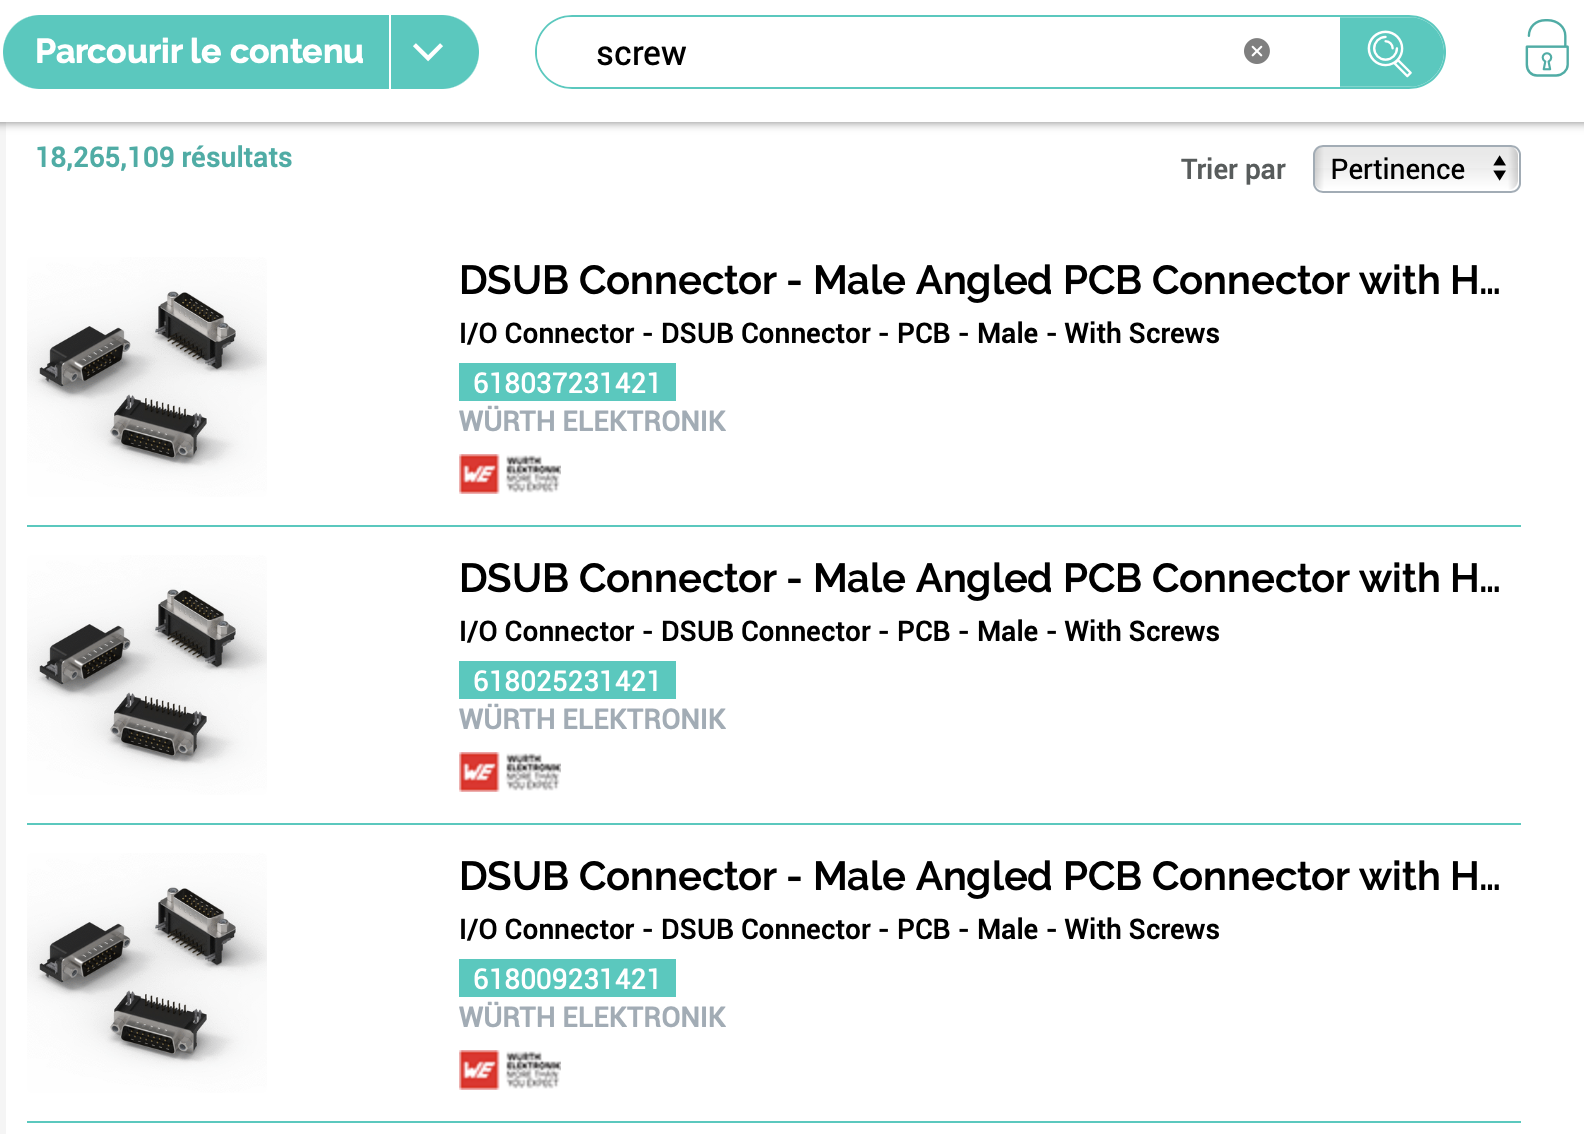
\includegraphics[width=.96\linewidth]{../../resources/se_test_screw.png}
		\caption{SE queried with ``screw''}
		\label{fig:test_es_screw}
	\end{subfigure}%
	\begin{subfigure}{.5\textwidth}
		\centering
		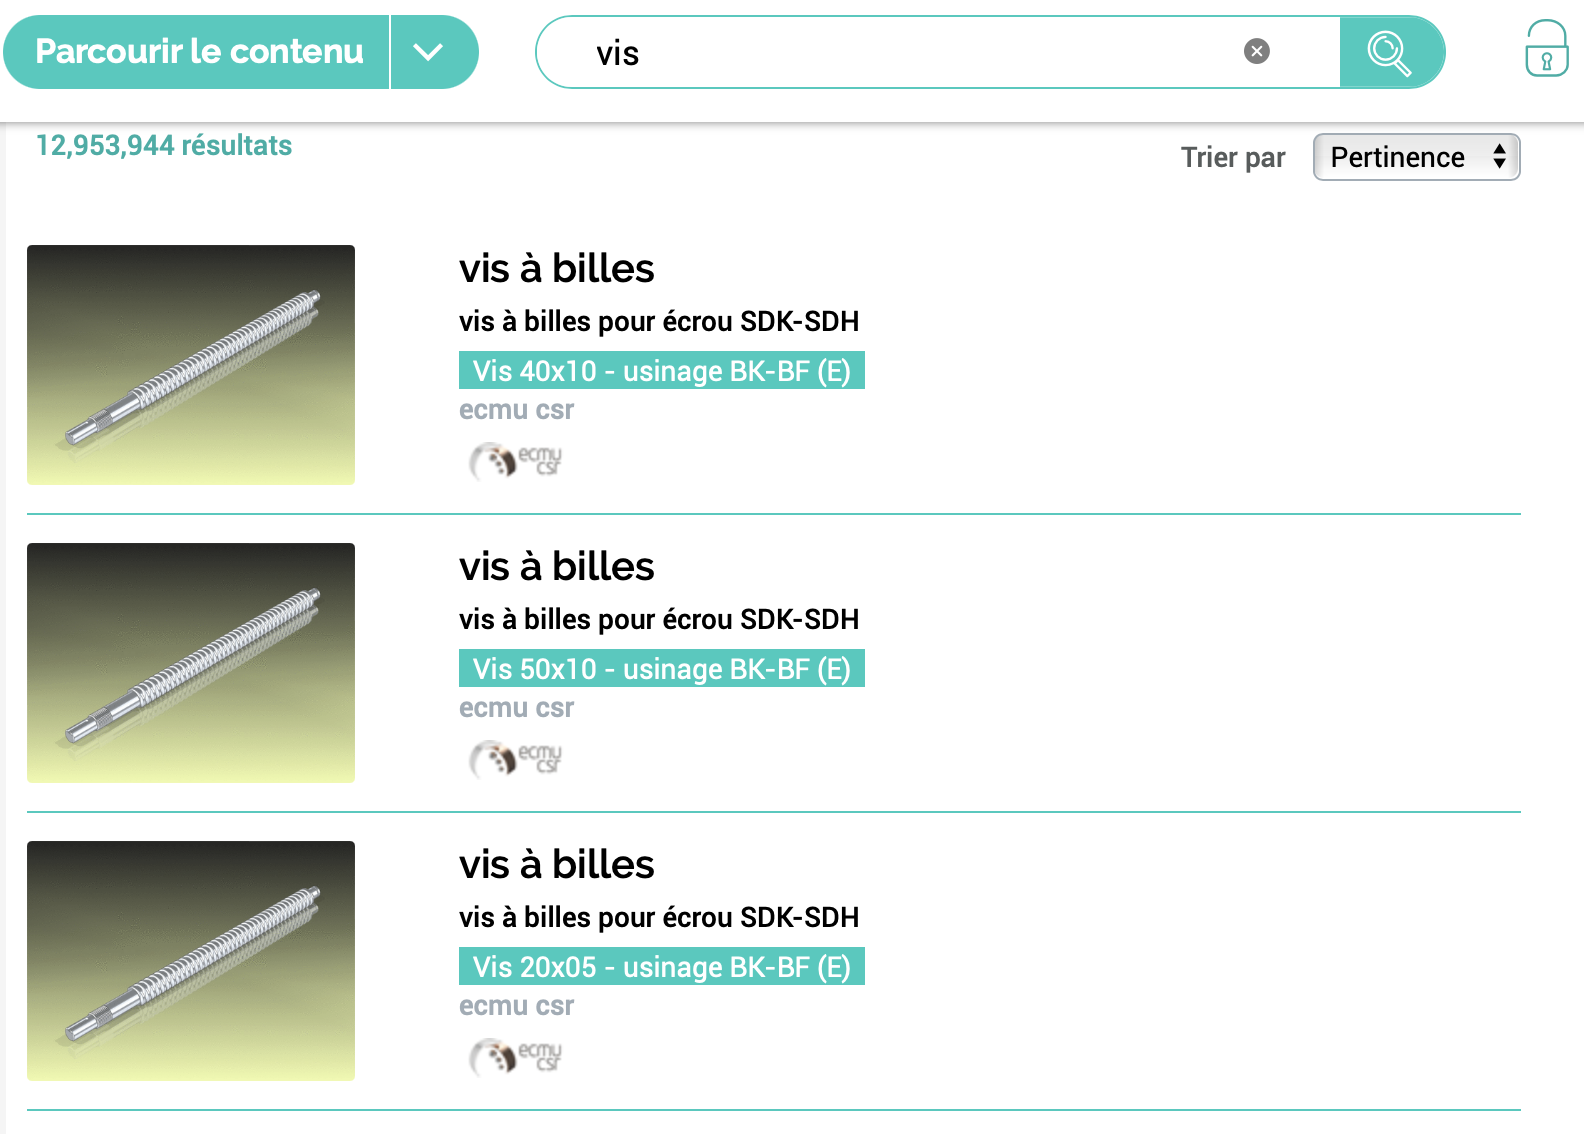
\includegraphics[width=.96\linewidth]{../../resources/se_test_vis.png}
		\caption{SE queried with ``vis''}
		\label{fig:test_es_vis}
	\end{subfigure}
	\caption{Example queries on TraceParts SE}
	\label{fig:tp_se_test}
\end{figure}

\paragraph{Research questions.}
Although ElasticSearch is well-known for its capabilities for fast textual searchess across the 
database entities, we believe that it is not an efficient use of the database to throw a bunch of 
words at it, which can be typed in different languages or formats according to different standards, 
and expect it to fetch satisfactory results. Such a search engine would fail to provide useful and 
proper web resources in so many easily imaginable cases shown below:

\begin{enumerate}
	\item What if the database contained the word ``screw'' but not ``vis''\footnote{``La vis'' means 
		a screw in French.}?
	\item What if the database contained screws but with no proper understanding of the dimensionality 
		of screws?
	\item What if the user query was like ``screwdriver used for small size screws'' and the database 
		had no understanding of whether the user was looking for wrenches, screws, or everything which 
		can be described as small-sized?
\end{enumerate}

The issues mentioned above are the by-product of performing only raw text-based searches across the 
database entities. It is not hard to imagine that some of the entities may contain the same words 
such as ``small'', ``medium'', ``large'', ``dimension'', ``standard'', ``colored'' and so on. Main 
research questions include ``how to make search engines understand necessary distinctions between 
products, products described in their descriptions, their attributes, languages that they are 
expressed in?'', ``what data structure(s) should be used to store data?'', ``how to develop 
algorithms/software to deal with these problems?''.

\paragraph{Research methodology.}
Currently, the search process is blindfolded, meaning that it has no idea what to look for in terms of 
concepts that matter to the user. To avoid such inefficiencies in the run-time performance and ranking 
of the search engine result pages, we can guide the search process by using ontologies and/or 
knowledge graphs \cite{reinanda2020knowledge,dietz2018utilizing,chen2020review}. Knowledge acquisition 
plays a crucial role in the process of developing 
ontologies and/or knowledge graphs. Several approaches to address some of the issues related to 
knowledge acquisition bottlenecks as well as information retrieval systems and search engine 
optimization strategies are demonstrated in chapter \ref{chap:literature}. In this thesis work, 
several knowledge acquisition strategies 
are described for introductory purposes for the following sections. My main contributions in this 
project include the development of a software architecture, implementation of different processing 
paradigms, and building a knowledge acquisition pipeline all of which are introduced and discussed 
thoroughly in chapter \ref{chap:development}. To acquire knowledge from the relational database of 
TraceParts, a relatively simple ontology has been developed and used to build the ultimate knowledge 
graph. The ontology and knowledge graph building process have been described in a more detailed 
fashion later on in the same chapter. In chapter \ref{chap:results_discussions}, implemented library 
and the final software as well as several tests are discussed. Finally, I share my conclusions on 
this project and the internship experiences in chapter \ref{chap:conclusions}.

\paragraph{Practical significance of the thesis.}
The goal of this project work has been dedicated to develop a PoC system with which we could test 
different hyphothesis and compare benchmark results relatively quickly and easily. Such a system would 
play the foundational role in the ultimate search engine version and be sufficient for further 
improvements step-by-step, iteratively.


\chapter{Literature Review}							% 2 pages
\label{chap:literature}
Information Retrieval (IR) is a process of obtaining relevant information from a database according to 
the given query. User queries are usually provided in a text format, however, there is no theoretical 
limit or restriction for other formats. IR systems should not be confused with database systems; 
although they perform searching processes on entities(i.e., documents), the key difference remains in 
the ranking process. Ranking documents to compute their relevancy is required by the IR system and 
therefore, it may be the case that the system will output results that do not match the query. In 
contrast, classical databases search for and output documents that always match the given query.

Different models can be used by IR systems. Although the strategies differ, the main goal 
is always to find the most relevant information \cite{baeza1999modern,brin1998anatomy}. 
To achieve this goal, the models transform documents 
into an appropriate representation and this is where different models can utilize different 
representations. There are three types of models which are shown below:

\begin{enumerate}
	\item \textit{Set-theoretic}. 
		Models of this type use the set representation to describe documents; a document can be viewed 
		as a set of phrases, words or even letters. Operations used to find similarities are set 
		operations.
	\item \textit{Algebraic}.
		Such models usually use vector or matrix representation for documents and the similarity 
		between the given query and a document is a scalar value yielded by some relevant algebraic 
		operation(i.e., dot product for vectors).
	\item \textit{Probabilistic}.
		The core idea behind these models is the probabilistic inference used for document retrieval. 
		Baye's theorem \cite{enwiki:1094315386} plays a very important role for such models. Similarities 
		are computed as a probability for the relevancy of a document if given a query.
\end{enumerate}

Some of the most popular search engines that have been able to utilize IR systems more than others are 
\textit{Google}, \textit{YouTube}, \textit{Amazon}, \textit{Microsoft Bing}, and so on. However, such 
big companies usually develop relatively very complex systems that are the best fit for very large-scale  
problems. Although most of such systems are commercially available, it may be too much of an overhead 
to try to adapt and use them in small or medium-scale projects. Instead, one should try to observe 
the key concepts and come up with specialized methodologies or strategies which will maximize 
the expected outcome/value of the project.

Search Engine Optimization (SEO) is a process of efficiency of a search engine (SE) or website traffic 
by applying a set of methods such as indexing, crawling, cross linking, etc \cite{enwiki:1082522144}. 
There are different SEO methods used to attract more and more users to websites by providing more 
appropriately ranked content.

There are many SEs that consider little or no semantics to find relevant results for a given user 
query; most of these systems perform text-based searches across the database. Adding semantics in 
order to guide the search algorithms is not a new idea and has been implemented by many researchers. 
Lai et al. have developed a fuzzy ontology for their fuzzy search engine Fuzzy-Go \cite{6007378}. 
Their ontology uses fuzzy logic to represent semantic distances between tokens(i.e., keywords, words) 
which enables Fuzzy-Go to go beyond text-only search by also being able to consider the synonyms of 
terms. 

Modern SEs index contents of web pages by searching and matching the resources with the user query 
which is usually enriched by one or more Information Retrieval (IR) techniques. Some of the well-known 
IR techniques are the TF-IDF ranking model \cite{enwiki:1092578440} and 
PageRank \cite{enwiki:1094205204}. 
Bonino et al. have proposed an automatic search refinement mechanism based on ontology navigation for 
which computing semantic query refinement requires focalization and generalization 
\cite{bonino2004ontology}. 

% Source \cite{baeza1999modern}

Knowledge acquisition has always been a bottleneck for large-scale systems. Since such systems require 
a significant amount of human expert knowledge to operate, scalability becomes a problem. 
Tudorache et al. have developed a lightweight web-based knowledge acquisition tool and ontology editor 
called WebProt\'eg\'e \cite{tudorache2013webprotege}. They have adopted the infrastructure of 
Prot\'eg\'e which enables collaboration on the back-end and using Google Web Toolkit on the front-end. 
Although it is useful to have such knowledge acquisition tools, one downside is usually an intermediate 
interface through which human experts convey their knowledge. Currently, experts are required to 
have some degree of understanding in FoL\footnote{First-order logic} \cite{fitting2012first} to be 
able to express their knowledge of some domain. A subset of FoL is used by ontologies due to their 
reasoning capabilities \cite{pease2007first}.


\chapter{Development}								% 20 pages - should be Data and Methods for UFAZ
\label{chap:development}
\section{Data}

Only a limited amount of data has been provided by the company \textit{TraceParts} due to 
confidentiality. 
However, provided data has been enough to develop a methodology for, at least, a proof of concept. 
To be more specific about the provided dataset, 100 database instances have been accessed and loaded 
into the local machine environment. For this purpose, docker container(s) has been used to abstract 
the database service(s).

% \begin{figure}[H]
% 	\centering
% 	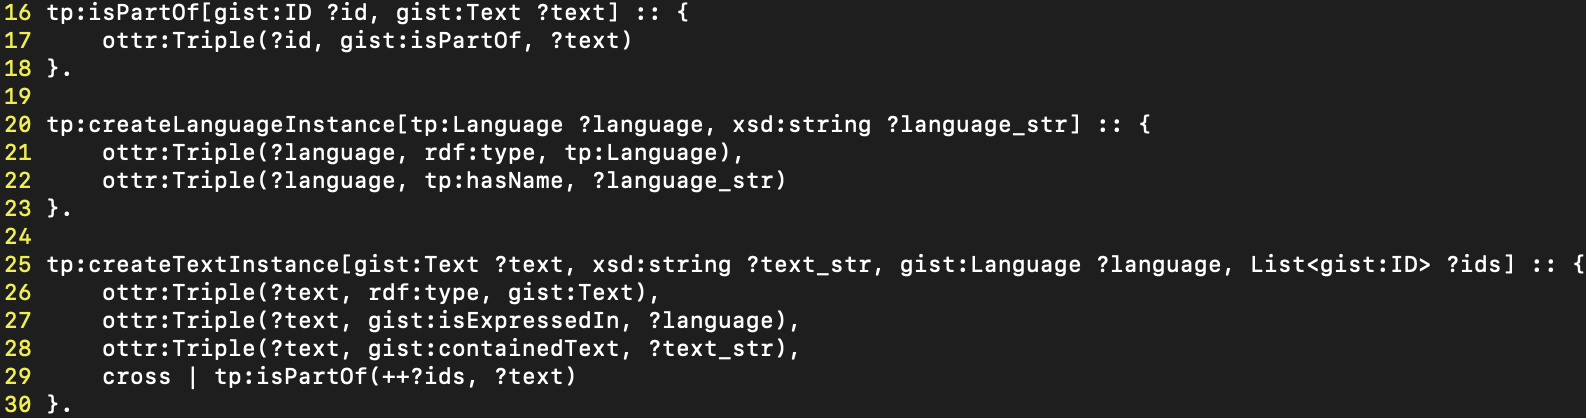
\includegraphics[width=0.75\textwidth]{../../resources/ottr_lib_example.png}
% 	\caption{ElasticSearch example}
% 	\label{fig:es_example}
% \end{figure}

\textit{ElasticSearch} (ES) is an open-source RESTful search and analytics engine which works in a 
distributed manner under the hood. It has been developed with Java and is based on Apache Lucene. 
In the ES database, data is stored with corresponding indices, and to retrieve it, we can send queries 
to its ``\lstinline{_search}'' endpoint. ES has many built-in functionalities such as filtering, 
ranking, aggregating, etc. However, we do not use any such functionalities in this project work since 
what we have been trying to achieve is a stand alone PoC system that contains all the necessary 
and customized functionalities for our use case.

\subsection{Database Schema}

The database has a somewhat complicated schema, however, there are several fields of interest for the 
matter of this internship. These fields include \textit{Part Family}, \textit{Part Number}, 
\textit{Part Family Name}, and \textit{Part Number Name}.

In the current version of the database used by the company, there are fields with the same values 
that are repeated in several places in the database memory. Such use of the service is probably 
inefficient in terms of memory complexity and maybe processing as well. In either case, there is 
inefficiency in the schema design.

\begin{table}[H]
	\centering
	\begin{tabular}{|p{0.25\textwidth}|p{0.20\textwidth}|p{0.23\textwidth}|p{0.23\textwidth}|}
		\hline
		\textbf{PartFamily} & \textbf{PartNumber} & \textbf{PartFamilyName} & \textbf{PartNumberName} \\
		\hline
		10-05112010-061898 & NSYMR34 & Telequick Mounting plate & Telequick Mounting plate 300X400 \\
		10-07032014-070631 & KTC2500ET32B & KT 3X2500CO FEEDER & KT 3X2500CO FEEDER LENGTH \\
		10-07032014-069644 & KTC1000lP7C1 & KT 5X1000CO FLAT ELBOW N1 & KT 5X1000CO FLAT ELBOW N1 \\
		10-19032018-083391 & LC1D12W7 & Contactor & Contactor - LC1D12W7 \\
		\hline
	\end{tabular}
	\caption{Example database instances}
	\label{tab:example_db_instances}
\end{table}

\section{Methods}

To make the TraceParts' search engine more semantic, the proposed solutions assume the existence of 
knowledge graph of database entities where there are relevant and useful semantic linkages between 
them. Since there is no such KG, I have proposed and implemented several solutions to fulfill this 
requirement. More specifically, I have worked on the Knowledge Acquisition part. The figure below 
illustrates the already-existing architecture of Knowledge Acquisition.

\begin{figure}[H]
	\centering
	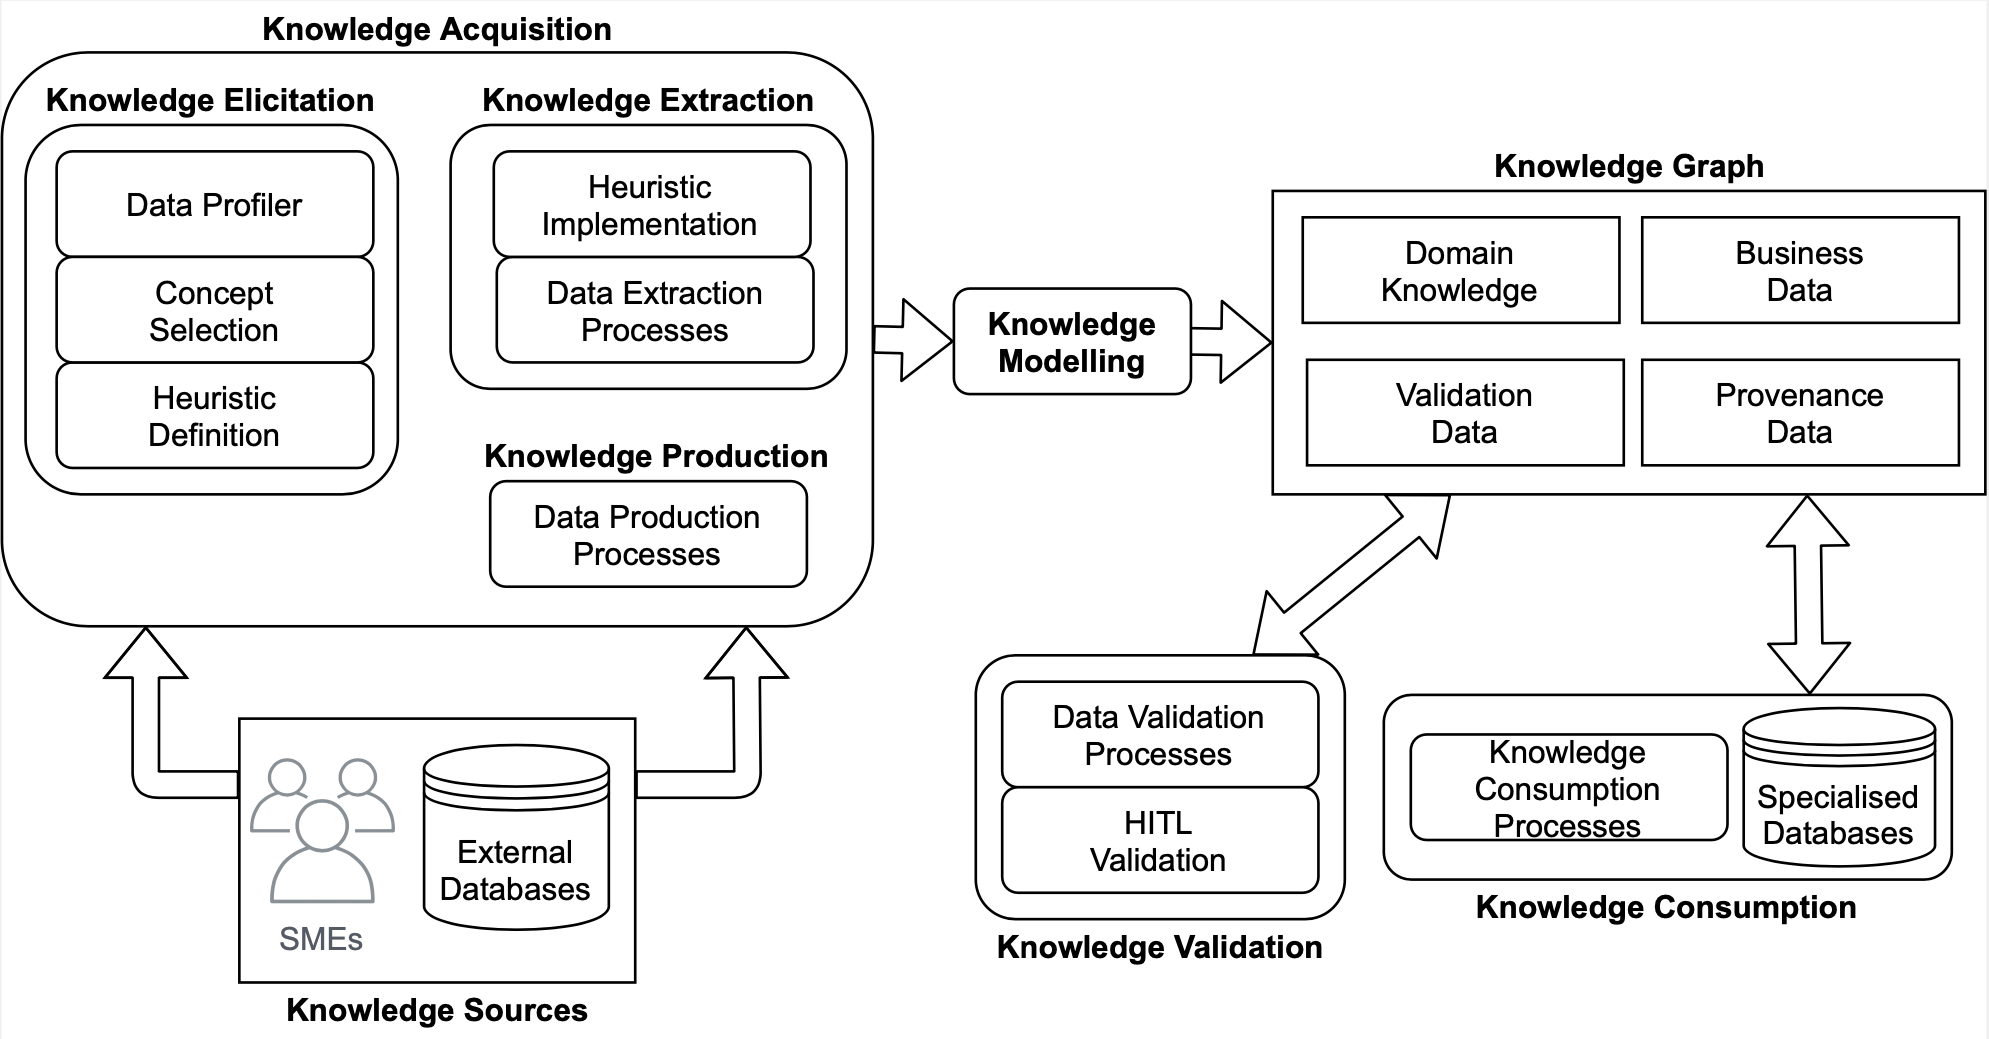
\includegraphics[width=0.75\textwidth]{../../resources/responding_pipeline.png}
	\caption{Knowledge Acquisition pipeline}
	\label{fig:responding_knowledge_acquisition_pipeline}
\end{figure}

In this figure, round-shaped rectangular boxes indicate the processes and sharp-shaped boxes indicate 
the storage. \textit{Knowledge elicitation}, \textit{knowledge extraction}, and \textit{knowledge 
consumption} are the three parts of the knowledge acquisition process.

Knowledge elicitation is the process of acquiring tacit knowledge from domain experts in the formal 
form. Conversion of tacit knowledge or insights into tangible and structured data is not trivial 
work and needs to be dealt with at the very first step of the project. 
Knowledge extraction is the process of extracting knowledge from (un)structured data containers. As 
an example of such a process, \textit{Extract-Transform-Load} (\textit{ETL}) can be given where data 
is extracted from one or more databases, then transformed in some specific way to be suitable for 
further use, and finally, loaded into one or more databases.
Knowledge production and consumption processes define how the linked data points are produced and 
requested by the end-users respectively. 

Knowledge validation is the process of KB\footnote{Knowledge Base} verification and 
evaluation \cite{LAUR,Owoc1999}. Knowledge verification focuses on the structural correctness of 
knowledge bases whereas evaluation takes care of the inference part so that only correct conclusions 
can be made within the knowledge base. There are several approaches for KB verification that are 
based on dependency tables, decision trees, machine learning, graphs, etc., and another set of 
approaches for evaluation is aimed at refinement, testing, generating, and so on.

Knowledge sources are where we acquire knowledge. These sources can either be subject-matter 
experts (SMEs) or some external databases. In the case of this project, we have used TraceParts' 
ElasticSearch database to extract knowledge, transform it to make it comply with the developed 
ontology, and load it into the Jena graph database. Throughout the rest of the processes, the only 
knowledge source has been the KG that we have acquired. This also helps us to simplify the 
knowledge validation steps since we only consider our KG as a unified source of truth and every other 
process, if needed, is built on top of this single knowledge source.

A knowledge graph is a data structure that represents some specific piece of knowledge by using 
graphs. In the context of KGs, nodes or vertices of the graph represent the concepts while edges or 
arcs represent the relationships between them. The distinction between ontologies and knowledge graphs 
is not still clear among many people. According to some sources, ontologies are only to represent 
concepts 
and relationships between those concepts whereas knowledge graphs also incorporate individuals or 
instances. However, this definition is also controversial among some other sources; for example, 
an ontology can also incorporate individuals or objects according to \cite{enwiki:1085831526}.

Although there are many debates on definitions of ontologies and knowledge graphs, I think that it may 
be a bit deviating route to take to define something whose whole purpose, ironically, is to define things. 
The reason behind this thought is that I do not think that every ``thing'' is clearly and rigorously 
definable. For example, even the concept of a ``straight line'' is not rigorously definable in the 
sense 
that its definition would not contain the concept of a straight line, or in other words, if circular 
definitions were not allowed then defining a ``straight line'' would not be possible at all and that is 
the reason it is accepted as a \textit{primitive} which is accepted to have no definition 
\cite{enwiki:1092767429}. The deeper reason for such things to happen, I think, is due to the nature of 
the language itself. We use language to describe or communicate our thoughts, feelings, emotions or 
experiences and these experiences are not inherently captured by the language itself. In fact, language is 
invented and learned by humans through an iterative process.

\subsection{Ontology Concerning The Search Engine}

The first important part of knowledge acquisition is to have an ontology describing the concepts and 
relationships between them in a formal way so that there is an agreed-upon structure of data. Developing 
an ontology is not an as easy job as it may sound. While designing an ontology, the designer should be 
aware of the implications of his/her design choices. Moreover, it is not a trivial task to be able to 
identify necessary and sufficient ontological objects (i.e, concepts and relationships). An ontology is 
considered well-designed if it is able to say what it is supposed to say and not say what it is not 
supposed to say. There is a balance between being less expressive to the degree that one cannot 
represent what is essential and more expressive to the degree that one can express a lot of things that 
are not meant to be essential. Either case is not considered good practice, in fact, it is the thin 
line that one should try to establish for the developed ontology \cite{cmariakeet}.

\begin{figure}[ht]
	\centering
	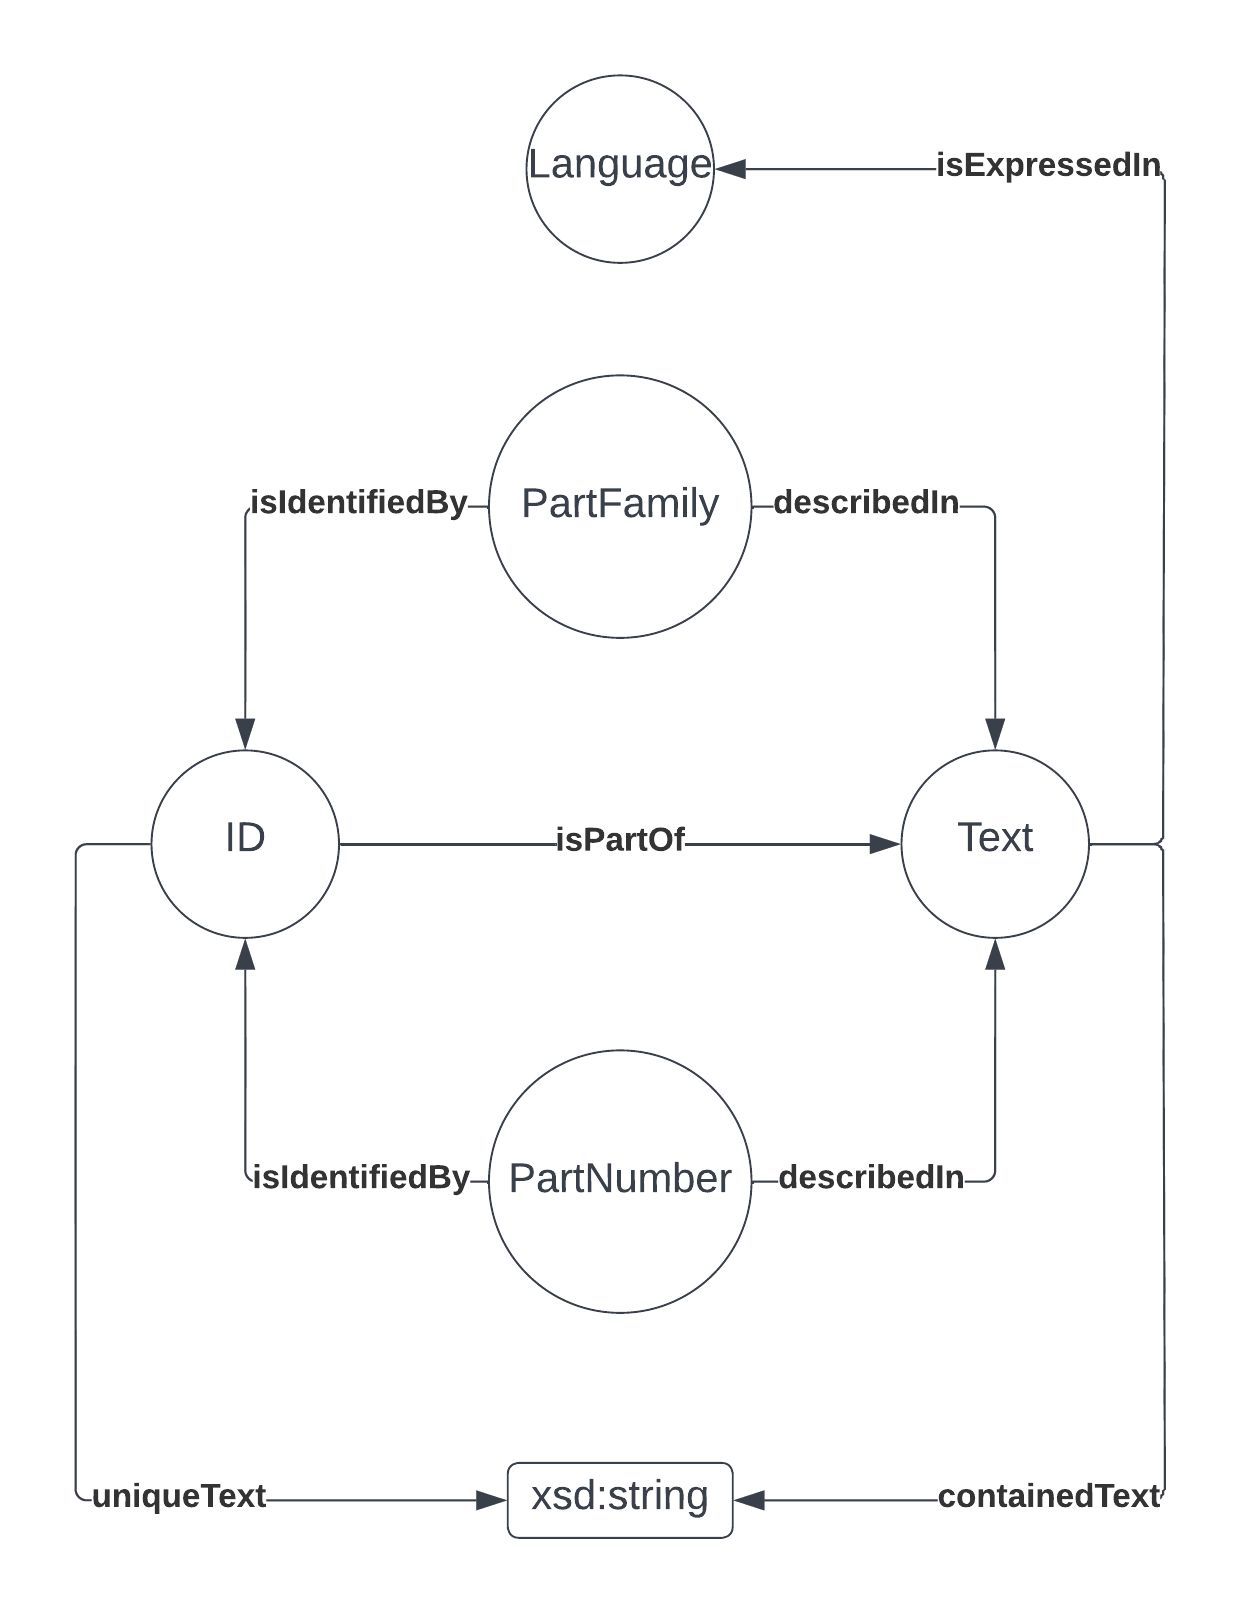
\includegraphics[width=0.70\textwidth]{../../resources/responding_se_onto.png}
	\caption{Ontology for knowledge acquisition relevant to the TraceParts' SE}
	\label{fig:ontology}
\end{figure}

In order to build a knowledge graph, one has to have \textit{T-box} and \textit{A-box}. These boxes are 
the essential parts of any knowledge graph. In the following sections, more specific details about 
these boxes and what T-box and A-box elements have been defined in this project are described 
thoroughly (see figure \ref{fig:ontology}). Since 
the reason for building ontologies and/or knowledge graphs is to have a unified vocabulary throughout 
the 
applications, we have also used another ontology called \textit{gist} \cite{gist} to integrate some of 
the concepts defined there that are useful for our purpose. Gist is an upper ontology that consists of 
business-related concepts with the least amount of ambiguity.

\paragraph{Concepts.}
Concepts are considered as \textit{terminology box} or \textit{T-box} elements and without them 
there is nothing to talk about since they define the concepts that can be used in the natural language. 
One can also think of T-box elements as classes defined in object-oriented programming. Table \ref{tab:ontology_concepts} demonstrates the ontological concepts used in the project with their descriptions and 
source ontology, if any, they have been taken from.\footnote{\textbf{tp} refers to the 
\textbf{T}race\textbf{P}arts ontology.}

\begin{table}[H]
	\centering
	\begin{tabular}{|p{0.20\textwidth}|p{0.35\textwidth}|p{0.25\textwidth}|}
		\hline
		\textbf{Concept name} & \textbf{Description} & \textbf{Integrated ontology} \\
		\hline
		ID & Used for unique identification (of Part Family/Number) & gist \\
		\hline
		Text & Used for textual descriptions (of Part Family/Number) & gist \\
		\hline
		PartNumber & Indicates a specific CAD model & -(tp) \\
		\hline
		PartFamily & Indicates a family/set of different CAD models & -(tp) \\
		\hline
		Language & Indicates the language of a given Text & gist \\
		\hline
	\end{tabular}
	\caption{Concepts}
	\label{tab:ontology_concepts}
\end{table}

\paragraph{Relations.}
Relations and individuals are the elements of \textit{assertion box} or \textit{A-box} and they play an 
essential role in linking the concepts with each other to get the complete knowledge. One can also think 
of A-box elements as objects declared in object-oriented programming. In table 
\ref{tab:ontology_relations}, relations(i.e., object and data properties), their domains/ranges, and 
the source ontology they have been taken from are shown.

\begin{table}[H]
	\centering
	\begin{tabular}{|p{0.20\textwidth}|p{0.35\textwidth}|p{0.25\textwidth}|}
		\hline
		\textbf{Relation name} & \textbf{Domain $\rightarrow$ Range} & \textbf{Integrated ontology} \\
		\hline
		uniqueText & ID $\rightarrow$ xsd:string & gist \\
		\hline
		containedText & Text $\rightarrow$ xsd:string & gist \\
		\hline
		isDescribedIn & PartNumber $\rightarrow$ Text & gist \\
		\hline
		isIdentifiedBy & PartFamily $\rightarrow$ ID & gist \\
		\hline
		isEpxressedIn & Text $\rightarrow$ Language & gist \\
		\hline
		isPartOf & ID $\rightarrow$ Text & gist \\
		\hline
		hasPartFamily & PartNumber $\rightarrow$ PartFamily & -(tp) \\
		\hline
	\end{tabular}
	\caption{Relations}
	\label{tab:ontology_relations}
\end{table}

\subsection{Developing OTTR Template Library}

Reasonable Ontology Templates (OTTR) is a specification on which arbitrary ontologies can be created. 
OTTR is useful due to its capabilities to handle templates. 

Templates can be of types either base or non-base. \textit{Base templates} are the ones whose body 
does not contain any \textit{non-base template} while the templates that are not of the base type 
can freely 
contain other non-base and base templates. The difference between the 2 types of templates is that 
a base template is replaced by its body after the compilation process while a non-base template is 
continuously replaced by its body until reaching the base template. According to the specification, a 
template consists of several parts and can be described as below:

\begin{lstlisting}
signature [ parameters ] :: {
	body
}.
\end{lstlisting}

The template body can contain another template signature with the relevant parameter list and during 
the compilation process, all the nested templates are exposed until reaching the base template. 
Below is shown a part of the developed OTTR library during the internship.

\begin{lstlisting}
tp:createIdInstance [ gist:ID? id, 
		xsd:str ?id_str ] :: {
	ottr:Triple(?id, rdf:type, tp:ID),
	ottr:Triple(?id, gist:uniqueText, ?id_str)
}.

tp:isPartOf [ gist:ID ?id, 
		gist:Text ?text ] :: {
	ottr:Triple(?id, gist:isPartOf, ?text)
}.

tp:createTextInstance [ gist:Text ?text, 
		xsd:string ?text_str, 
		gist:Langauge ?language, 
		List<gist:ID> ?ids ] :: {
	ottr:Triple(?text, rdf:type, gist:Text),
	ottr:Triple(?text, gist:isExpressedIn, ?language),
	ottr:Triple(?text, gist:containedText, ?text_str),
	cross | tp:isPartOf(++?ids, ?text)
}.
\end{lstlisting}

Once we have an OTTR library, we can use it to declare and use instances of our knowledge graph easily 
without even knowing about the underlying OTTR triples. This also allows us to build knowledge graphs 
in a more flexible way such that if we needed to change the underlying ontology, we would not have to 
go through each instance one by one in order to apply this modification throughout the whole graph. 
Instead, everything would be recompiled with the modified library and that is it. Even when writing a 
template library, we tend to build templates as modular as possible so that the code is easily 
maintainable. This is, in fact, due to the nature of templates and their compilation process. Since 
each non-base template gets replaced by its body, this process allows us to recursively use a 
hierarchy 
of templates which eases the developers' work very significantly.

\subsection{Software Architecture}

There are different paradigms that are used to develop robust software with the help of clear, 
simple, and intuitive architectures. Such software architectures usually tend to be modular by 
encapsulating low-level working principles of the software pieces. \textit{Clean architecture} is 
one of many software architecture design patterns that combine many useful aspects of different 
paradigms.

\begin{figure}[H]
	\centering
	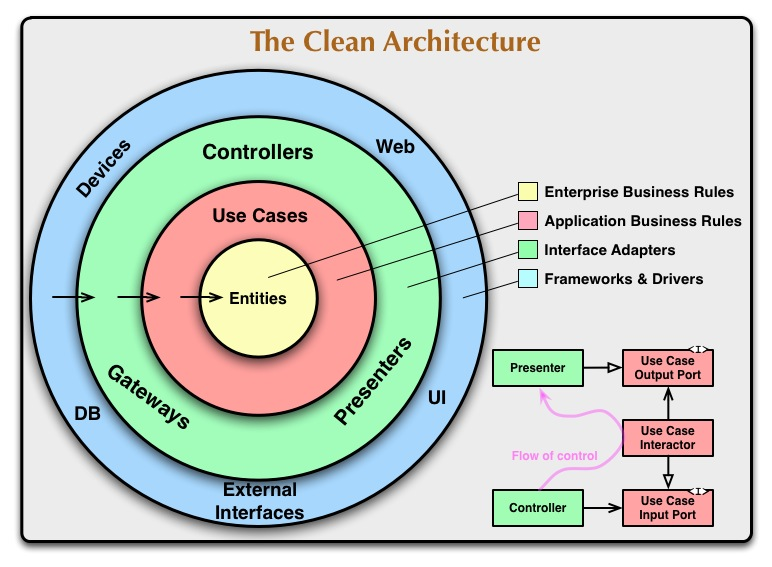
\includegraphics[width=0.7\textwidth]{../../resources/CleanArchitecture.jpeg}
	\caption{The Clean Architecture \cite{unclebob}}
	\label{fig:clean_arch}
\end{figure}

Figure \ref{fig:clean_arch} illustrates the clean architecture visually. Developing clean software 
architecture requires to comply with one important rule which is called the 
\textit{dependency rule}. The dependency rule states that any inner layer in the architecture may not 
depend on any outer layer while the opposite is possible and desired. To fulfill this rule, the most 
inner layer is called \textit{entities} and is to describe the most general or high-level business 
rules. Such rules are only business-dependent and have nothing to do with the rest of the developed 
software. Following this layer, comes the \textit{use cases}. Use cases define the same business rules 
on the application level which is to say, such implementation depends on the enterprise-wide business 
rules. \textit{Interface adapters} shown in the green circle are to serve as some sort of communication 
medium between the internal and external resources describing data format conversions. Finally, the 
most outer layer in the architecture is \textit{frameworks and adapters} which include third-party 
services such as databases, web frameworks, and so on. This layer contains the least amount of code 
development as well as a potential harm.

\paragraph{Diagrams.}
Figure \ref{fig:soft_arch} illustrates the UML class diagram with classes and relations between them. 
To get the top-down view, the most abstract or high-level classes are \textbf{ETL}, \textbf{ETLOperation} 
and \textbf{Data}. ETL may use zero or more ETLOperation and each such operation both consumes and 
produces OperationalData which is a subclass of the Data class. Each ETLOperation object is stored in 
the \textit{pipeline} attribute of an ETL object and the \textit{entity\_buffer} can be used for 
global data manipulations. It is the responsibility of the ETL object to keep track of termination 
condition(s) of the 
global program execution and not the ETLOperation objects. There are several private methods within 
the ETL to choose between the processing paradigms(i.e., sequential or parallel). A user of the 
library needs to create ETLOperation without directly interacting with it. In fact, ETLOperation is 
an abstract class with an unimplemented method \textit{run(\ldots)} as shown in the first row of table 
\ref{tab:abstract_methods} and for this purpose, there are three main subclasses of ETLOperation: 
\textbf{Extractor}, \textbf{Transformer} and \textbf{Loader}. All of these classes have also pure abstract 
methods \textit{extract(\ldots)}, \textit{transform(\ldots)} and \textit{load(\ldots)} respectively shown 
in the same table \ref{tab:abstract_methods}. This is to increase 
modularity, maintainability, and readability of the code by making sure that any ETLOperation is either of 
type Extractor or Transformer or Loader. One level down, there are also two classes that inherit from both 
the Extractor and Loader classes: \textbf{DatabaseOps} and \textbf{FileOps}. These two classes are used 
to abstract away two different extraction/loading paradigms(i.e., the ones that are local to the machine 
and the ones that need connectivity in the network). These operations can either be used for extraction or 
loading purposes with a single connection to a database or another machine and therefore, they inherit 
both the Extractor and Loader. The leaves of the class diagram contain the actual implementations of 
these methods and the user is able to initialize objects of these types.

\begin{figure}[H]
	\centering
	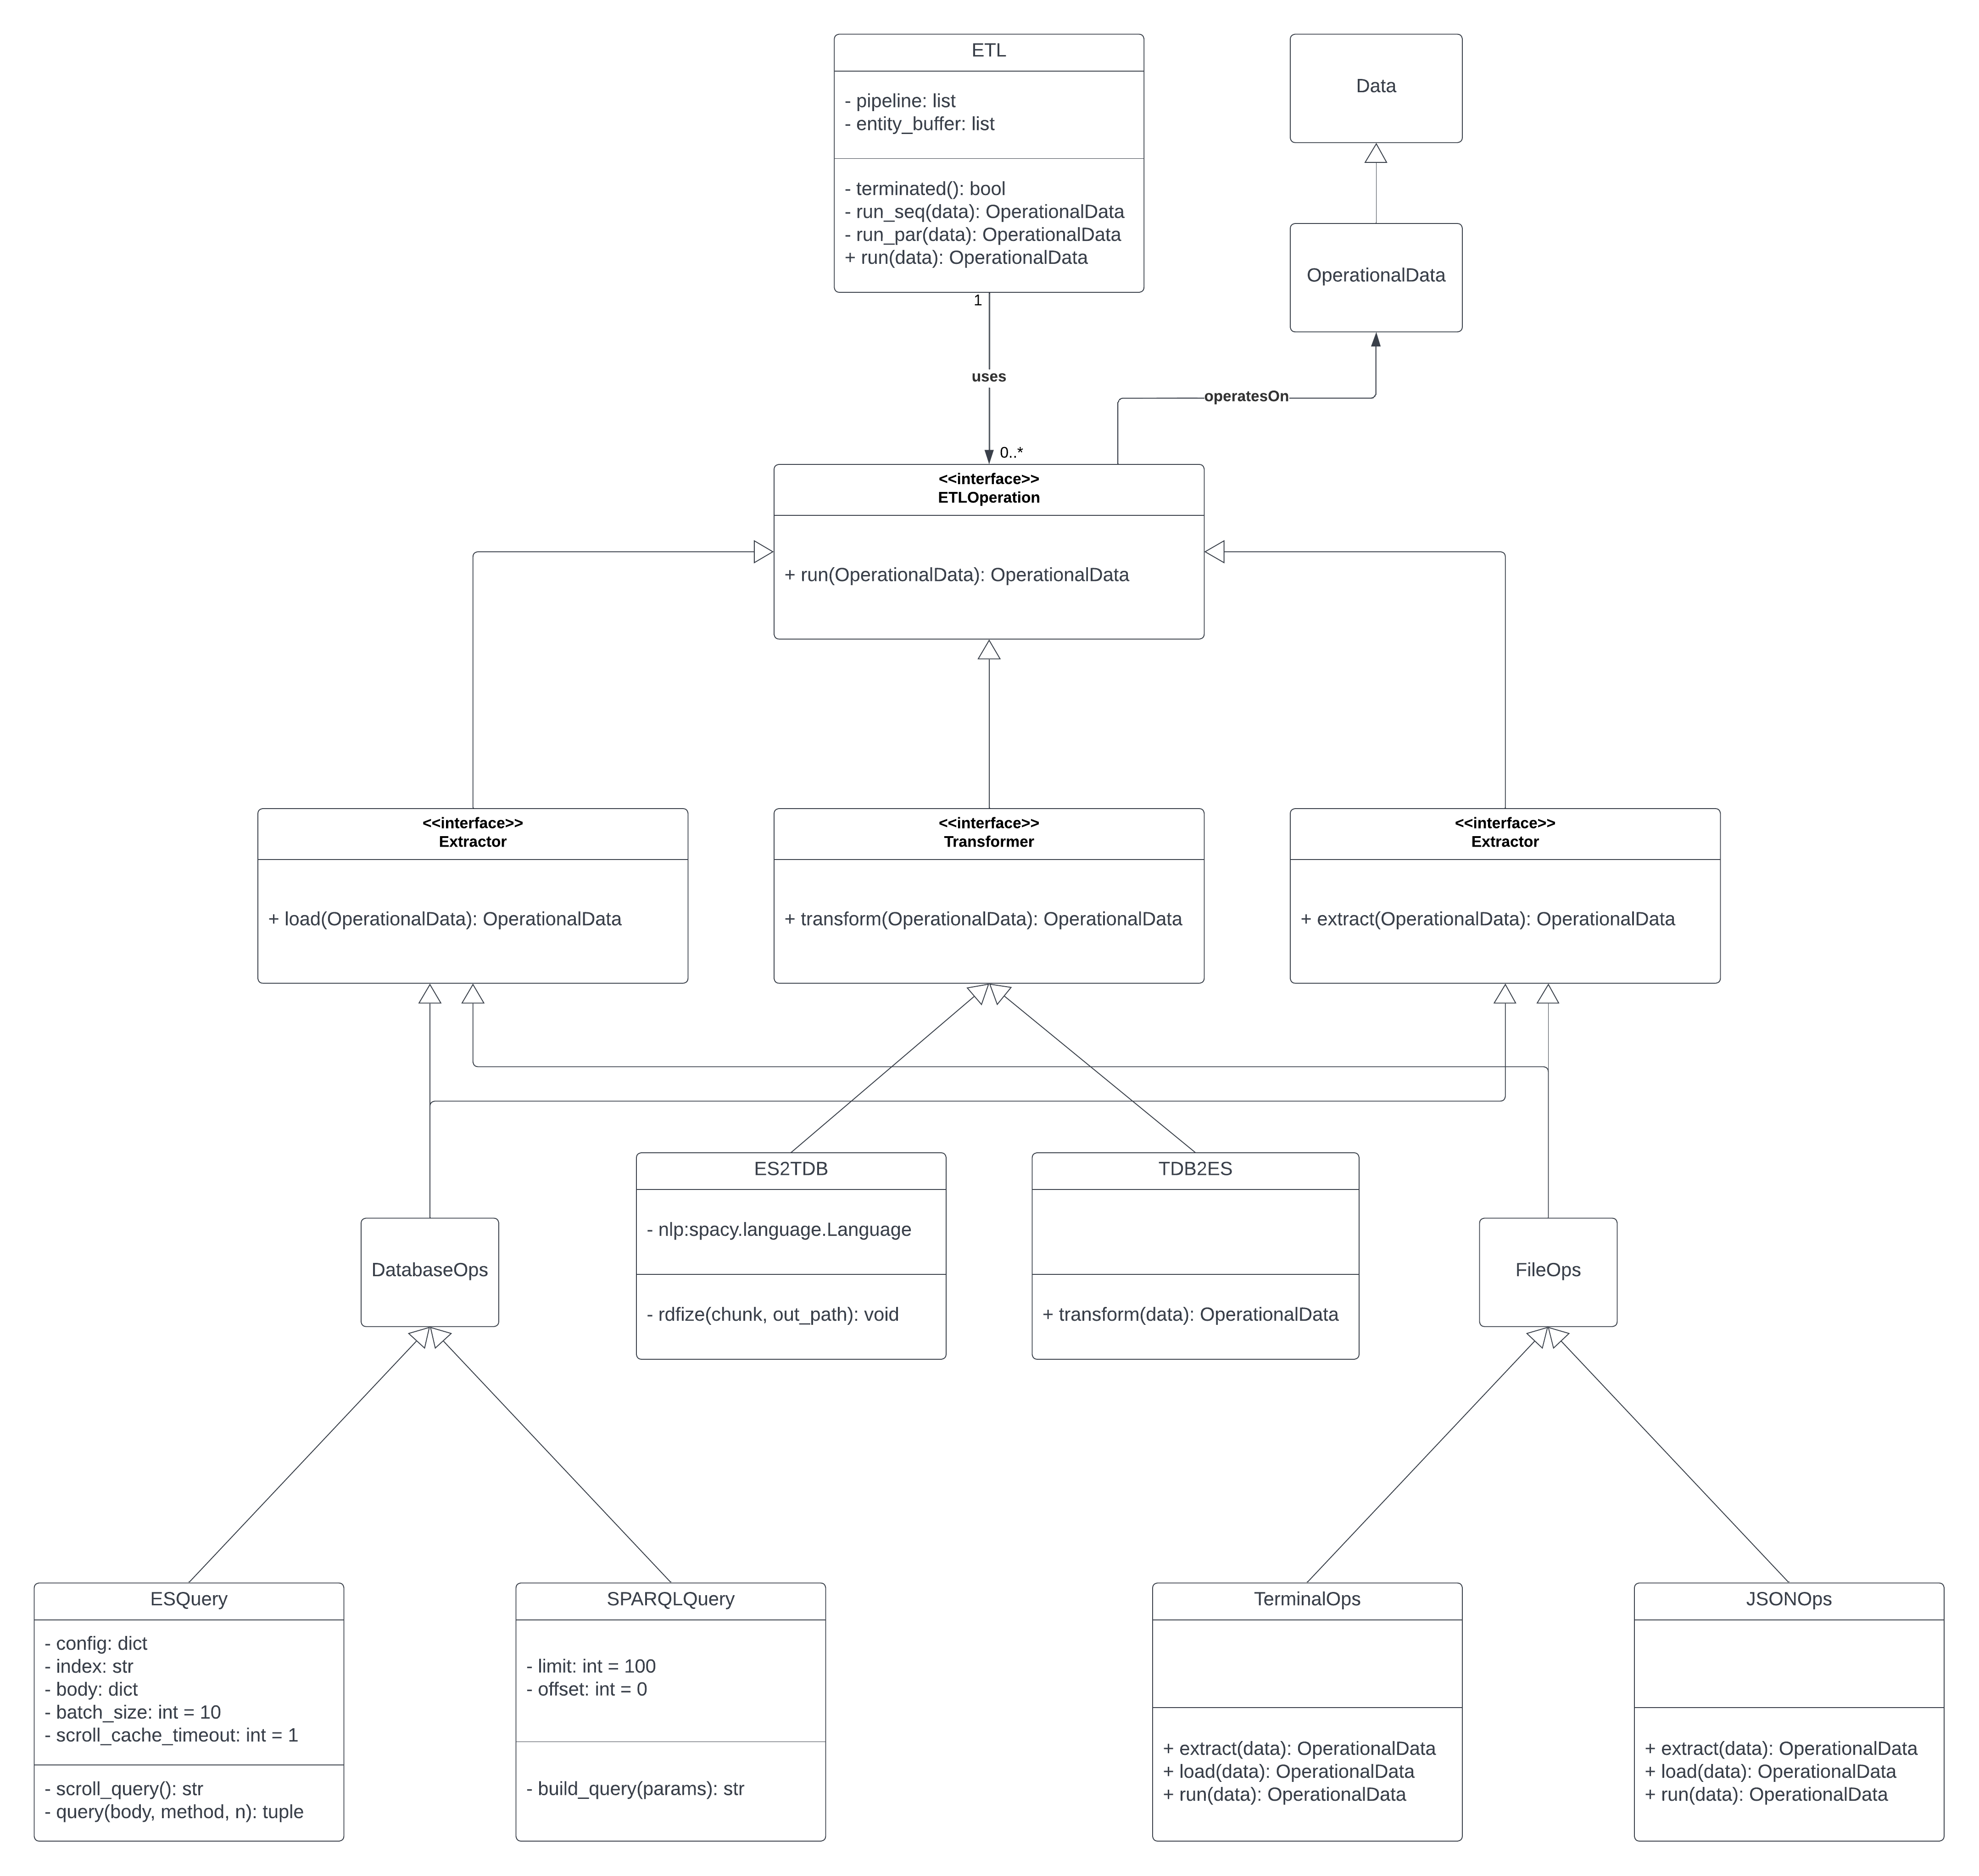
\includegraphics[width=0.95\textwidth]{../../resources/soft_arch.png}
	\caption{UML Class diagram}
	\label{fig:soft_arch}
\end{figure}

In case of any operational change in the business-logic level, one should be able to easily inherit his 
own \textit{implementation class}(i.e., the one which implements the abstract method(s) of its 
super/parent classes) from one or more of the top-level classes\footnote{The recommended classes to be 
inherited from are usually \textbf{DatabaseOps} and \textbf{FileOps} or \textbf{Transformer}.}. For 
example, if the database on which the KG is usually stored has to be changed to another database system, 
one can either modify the existing \textbf{SPARQLQuery} class or create a new, let's say, 
\textbf{MongoQuery} class inherited from Extractor and Loader. An instance of MongoQuery would be 
as easily 
usable as that of SPARQLQuery. This flexibility is due to the reason that this software architecture is 
very similar to and almost the same as the clean software architecture described previously; moving 
from the top of the hierarchy to the down is analogous to moving from the most inner circle to the 
most outer one in the clean software architecture.

\begin{table}[H]
	\centering
	\begin{tabular}{|c|c|}
		\hline
		\textbf{Class} & \textbf{Method} \\
		\hline
		ETLOperation & run(data: OperationalData) $\rightarrow$ OperationalData \\
		\hline
		Extractor & extract(data: OperationalData) $\rightarrow$ OperationalData \\
		\hline
		Transformer & transform(data: OperationalData) $\rightarrow$ OperationalData \\
		\hline
		Loader & load(data: OperationalData) $\rightarrow$ OperationalData \\
		\hline
	\end{tabular}
	\caption{Abstract methods}
	\label{tab:abstract_methods}
\end{table}

Users of this project are still the developers who are going to use \textit{knowledge acquisition} to 
make the resources semantically available for the final search engine processes. This being said, 
another type of user would be the end-users who are going to use/test the search engine by providing 
various textual queries and receiving the documents found and ranked by the search engine. Figure 
\ref{fig:soft_use_cases} demonstrate these use cases.

\begin{figure}[H]
\centering
\begin{subfigure}{.5\textwidth}
  \centering
  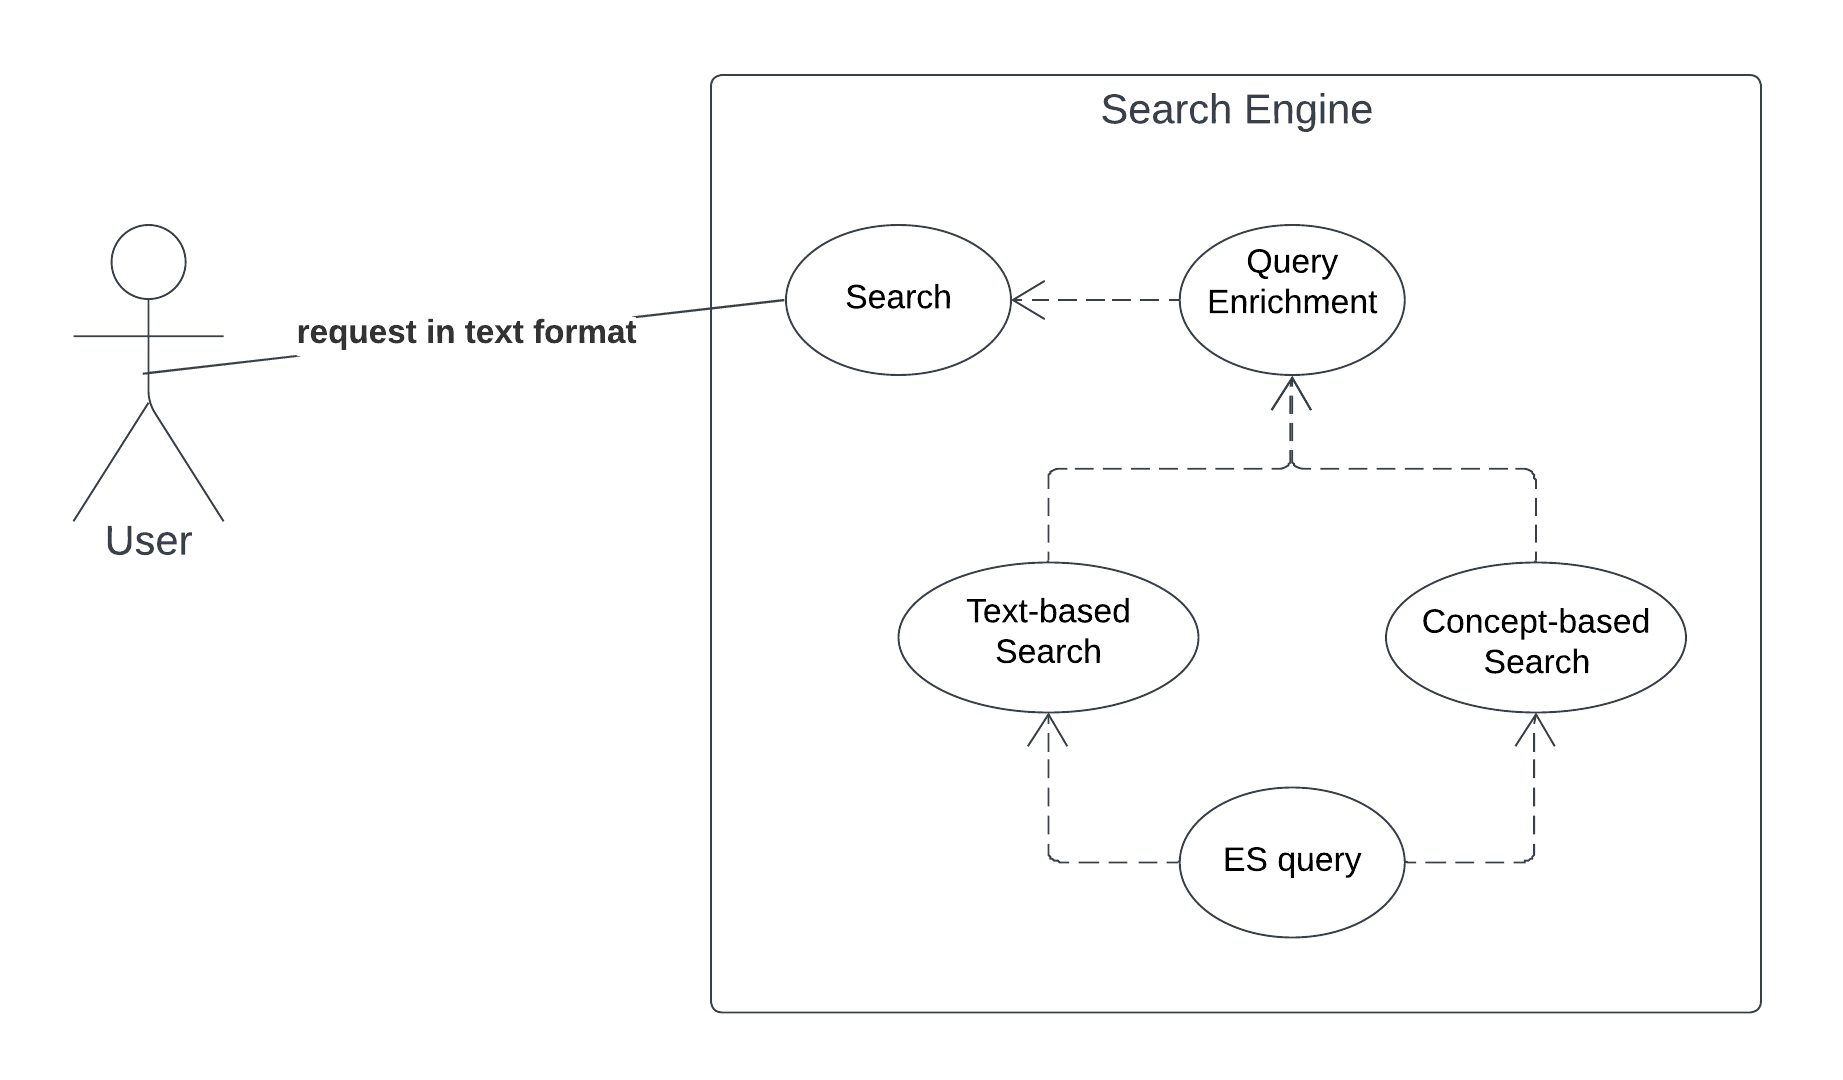
\includegraphics[width=.75\linewidth]{../resources/soft_use_case_1.png}
  \caption{Use case diagram for Knowledge Acquisition}
  \label{fig:subsoft_use_case_1}
\end{subfigure}%
\begin{subfigure}{.5\textwidth}
  \centering
  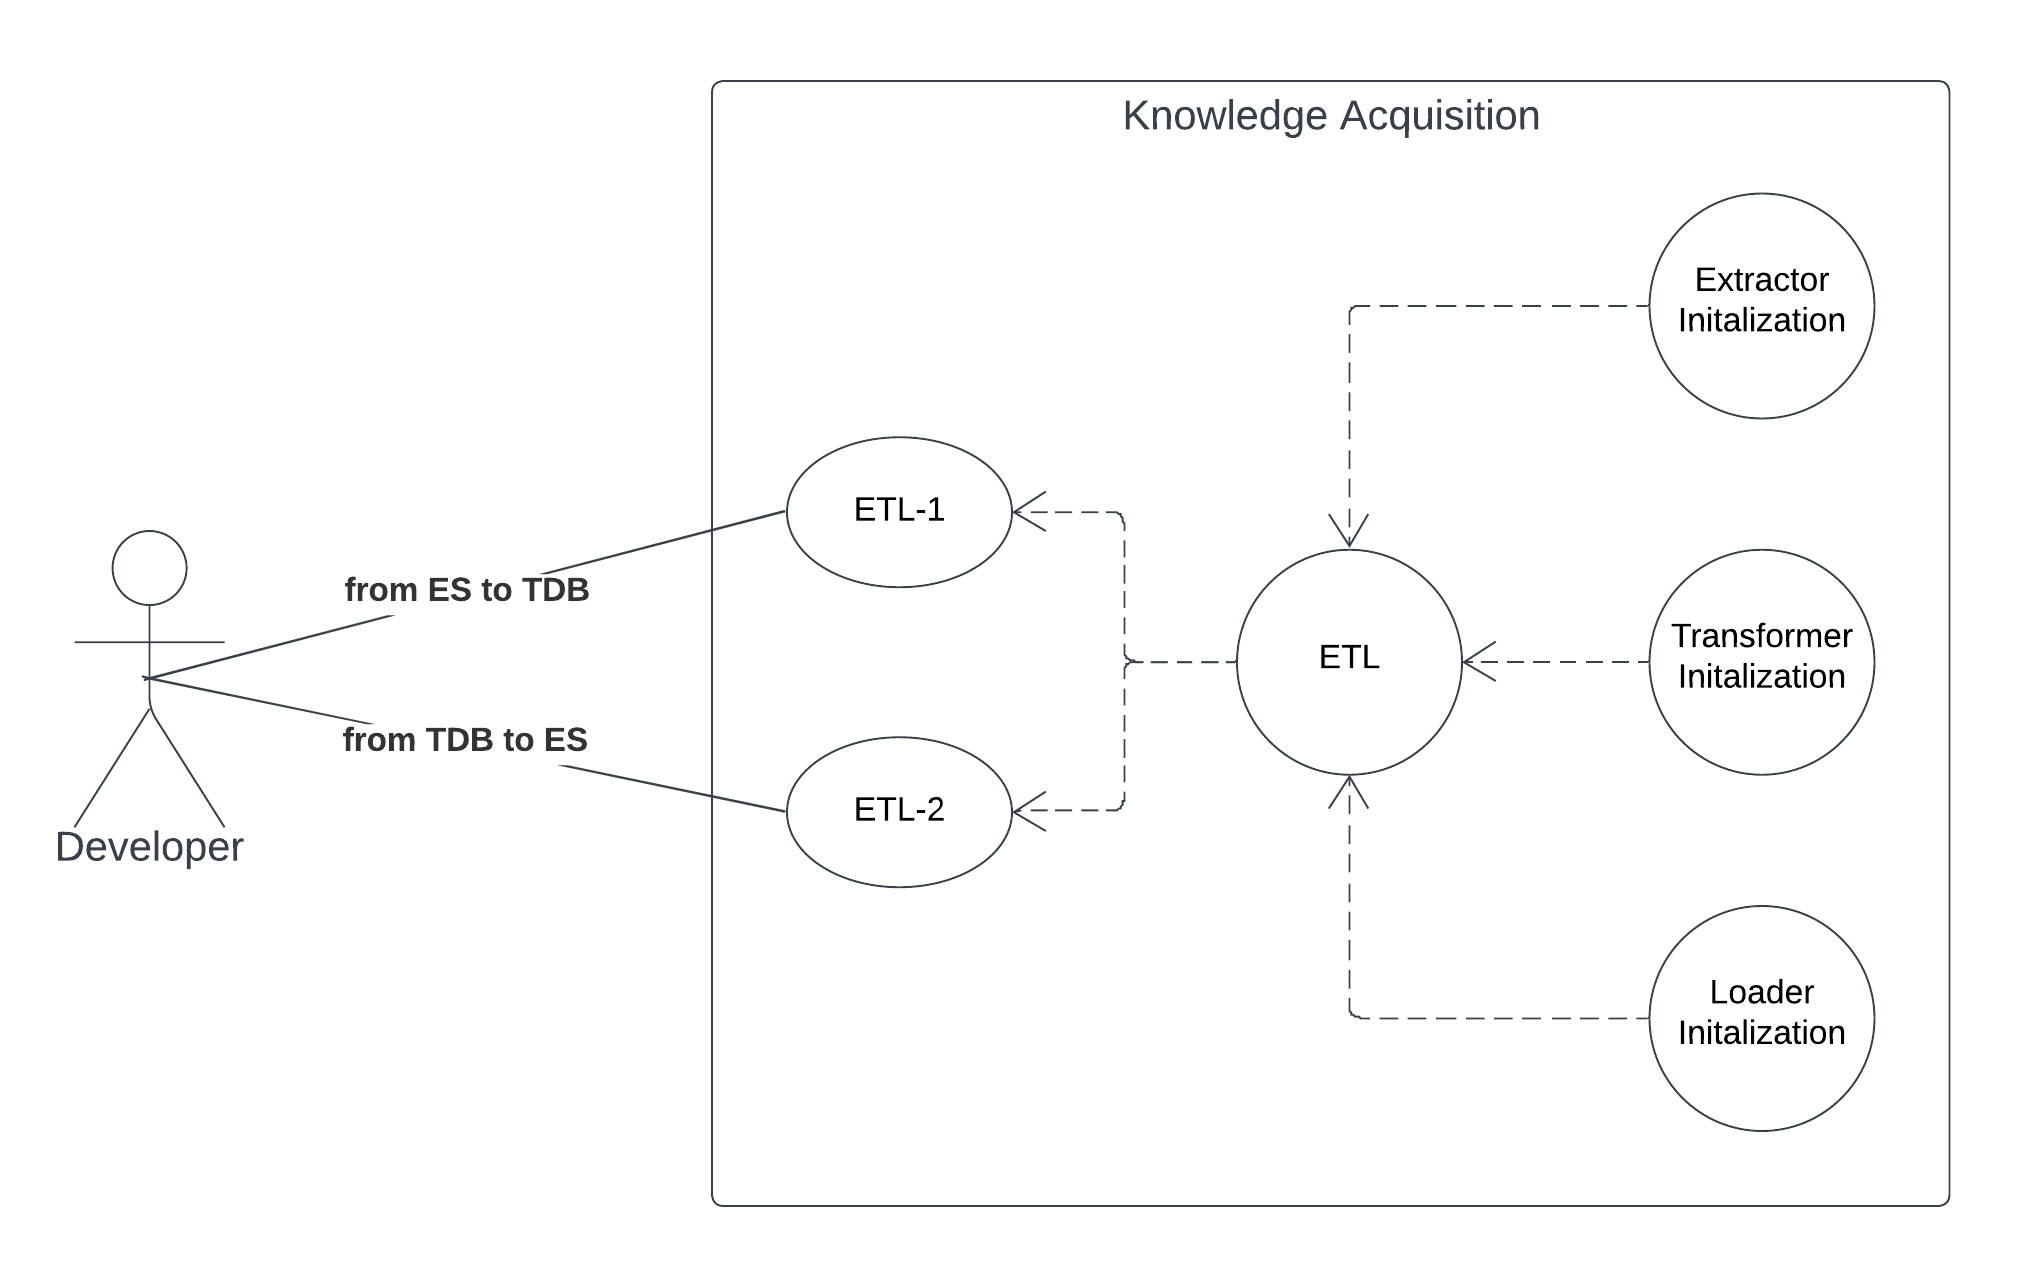
\includegraphics[width=.75\linewidth]{../resources/soft_use_case_2.png}
  \caption{Use case diagram for Search Engine}
  \label{fig:soft_use_case_2}
\end{subfigure}
\caption{Use case diagrams}
\label{fig:soft_use_cases}
\end{figure}

% Activity diagram is shown in tigure \ref{fig:soft_activity}.
% 
% \begin{figure}[H]
% 	\centering
% 	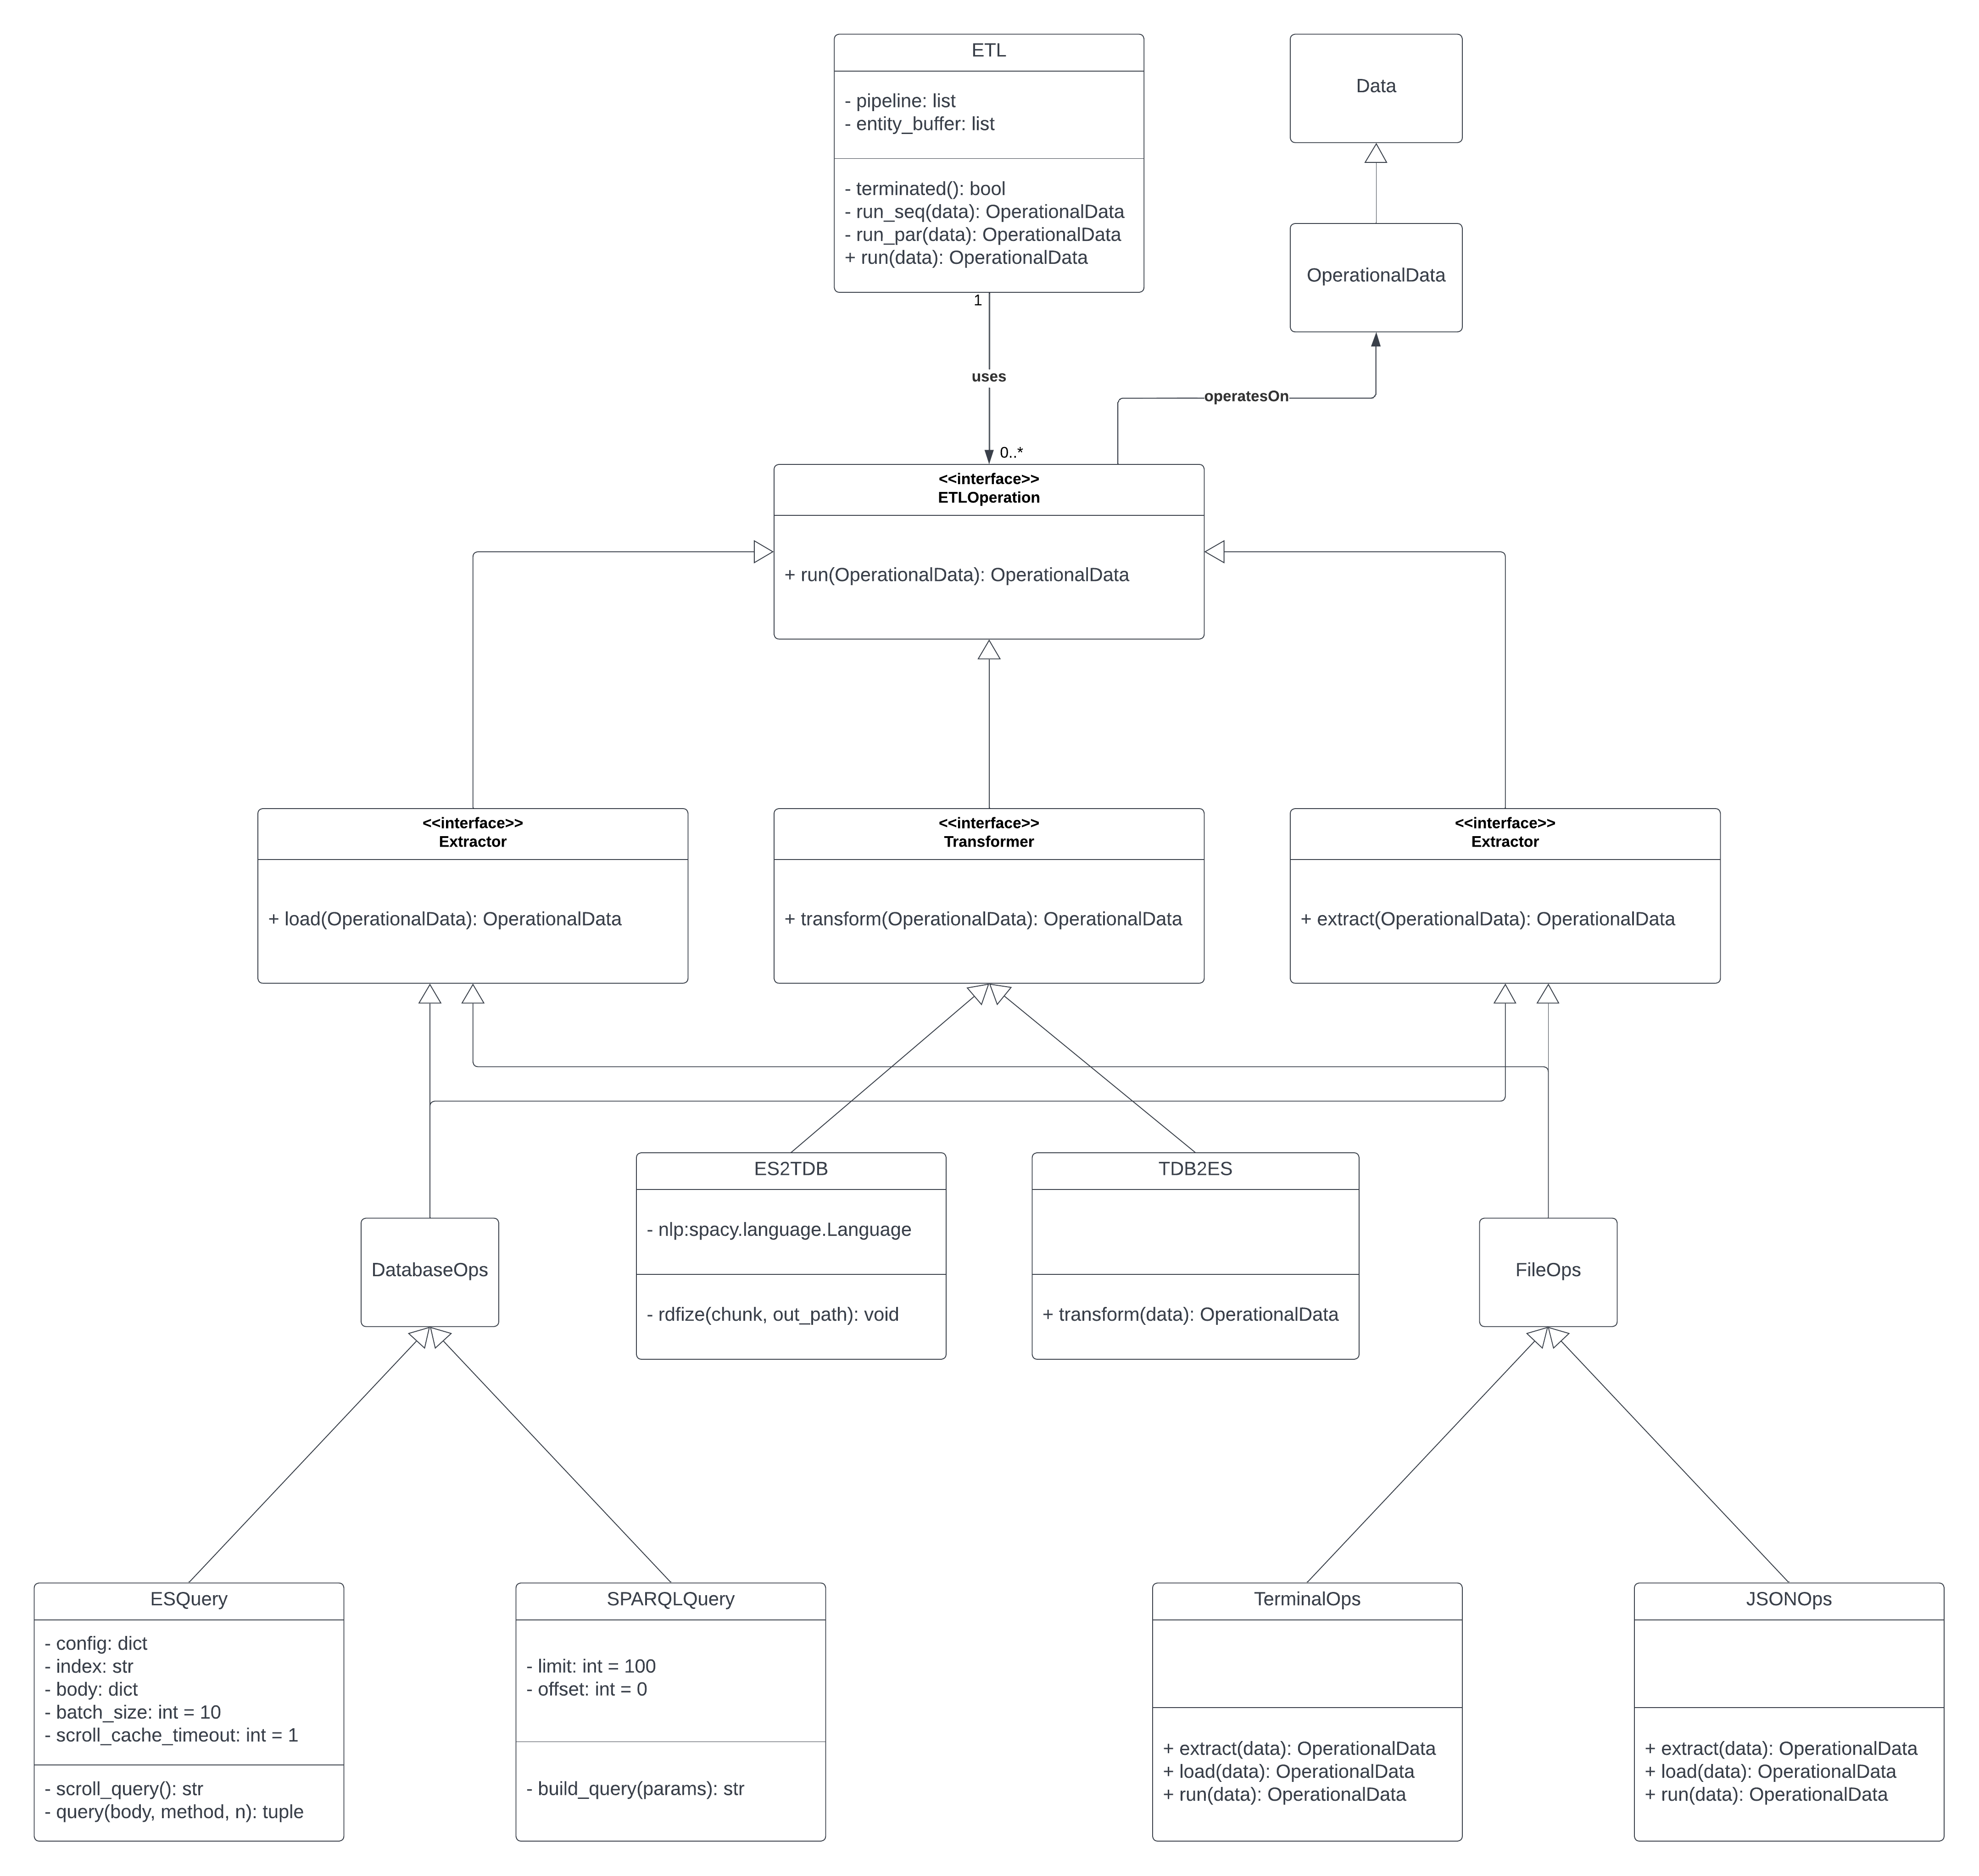
\includegraphics[width=0.75\textwidth]{../../resources/soft_arch.png}
% 	\caption{Activity diagram}
% 	\label{fig:soft_activity}
% \end{figure}

Interaction or sequence diagram is illustrated in figure \ref{fig:soft_sequence}. In order to 
perform ETL, three operations(i.e., Extractor, Transformer and Loader) are initialized. Extractor and 
Loader are usually required to create a session to be able to send requests to a database. An 
extractor 
object has an attribute called \textit{is\_active} which indicates if the most recent request was 
able to fetch some data. If nothing was fetched then this attribute is set to a boolean value of 
\textit{false}, otherwise, it is set to \textit{true}. The object of ETL class checks the value of 
\textit{is\_active} attribute of its first component(i.e., Extractor) in order to decide whether 
it should terminate or continue. If the termination criterion is not met then the residual 
components in the pipeline are executed.

\begin{figure}[H]
	\centering
	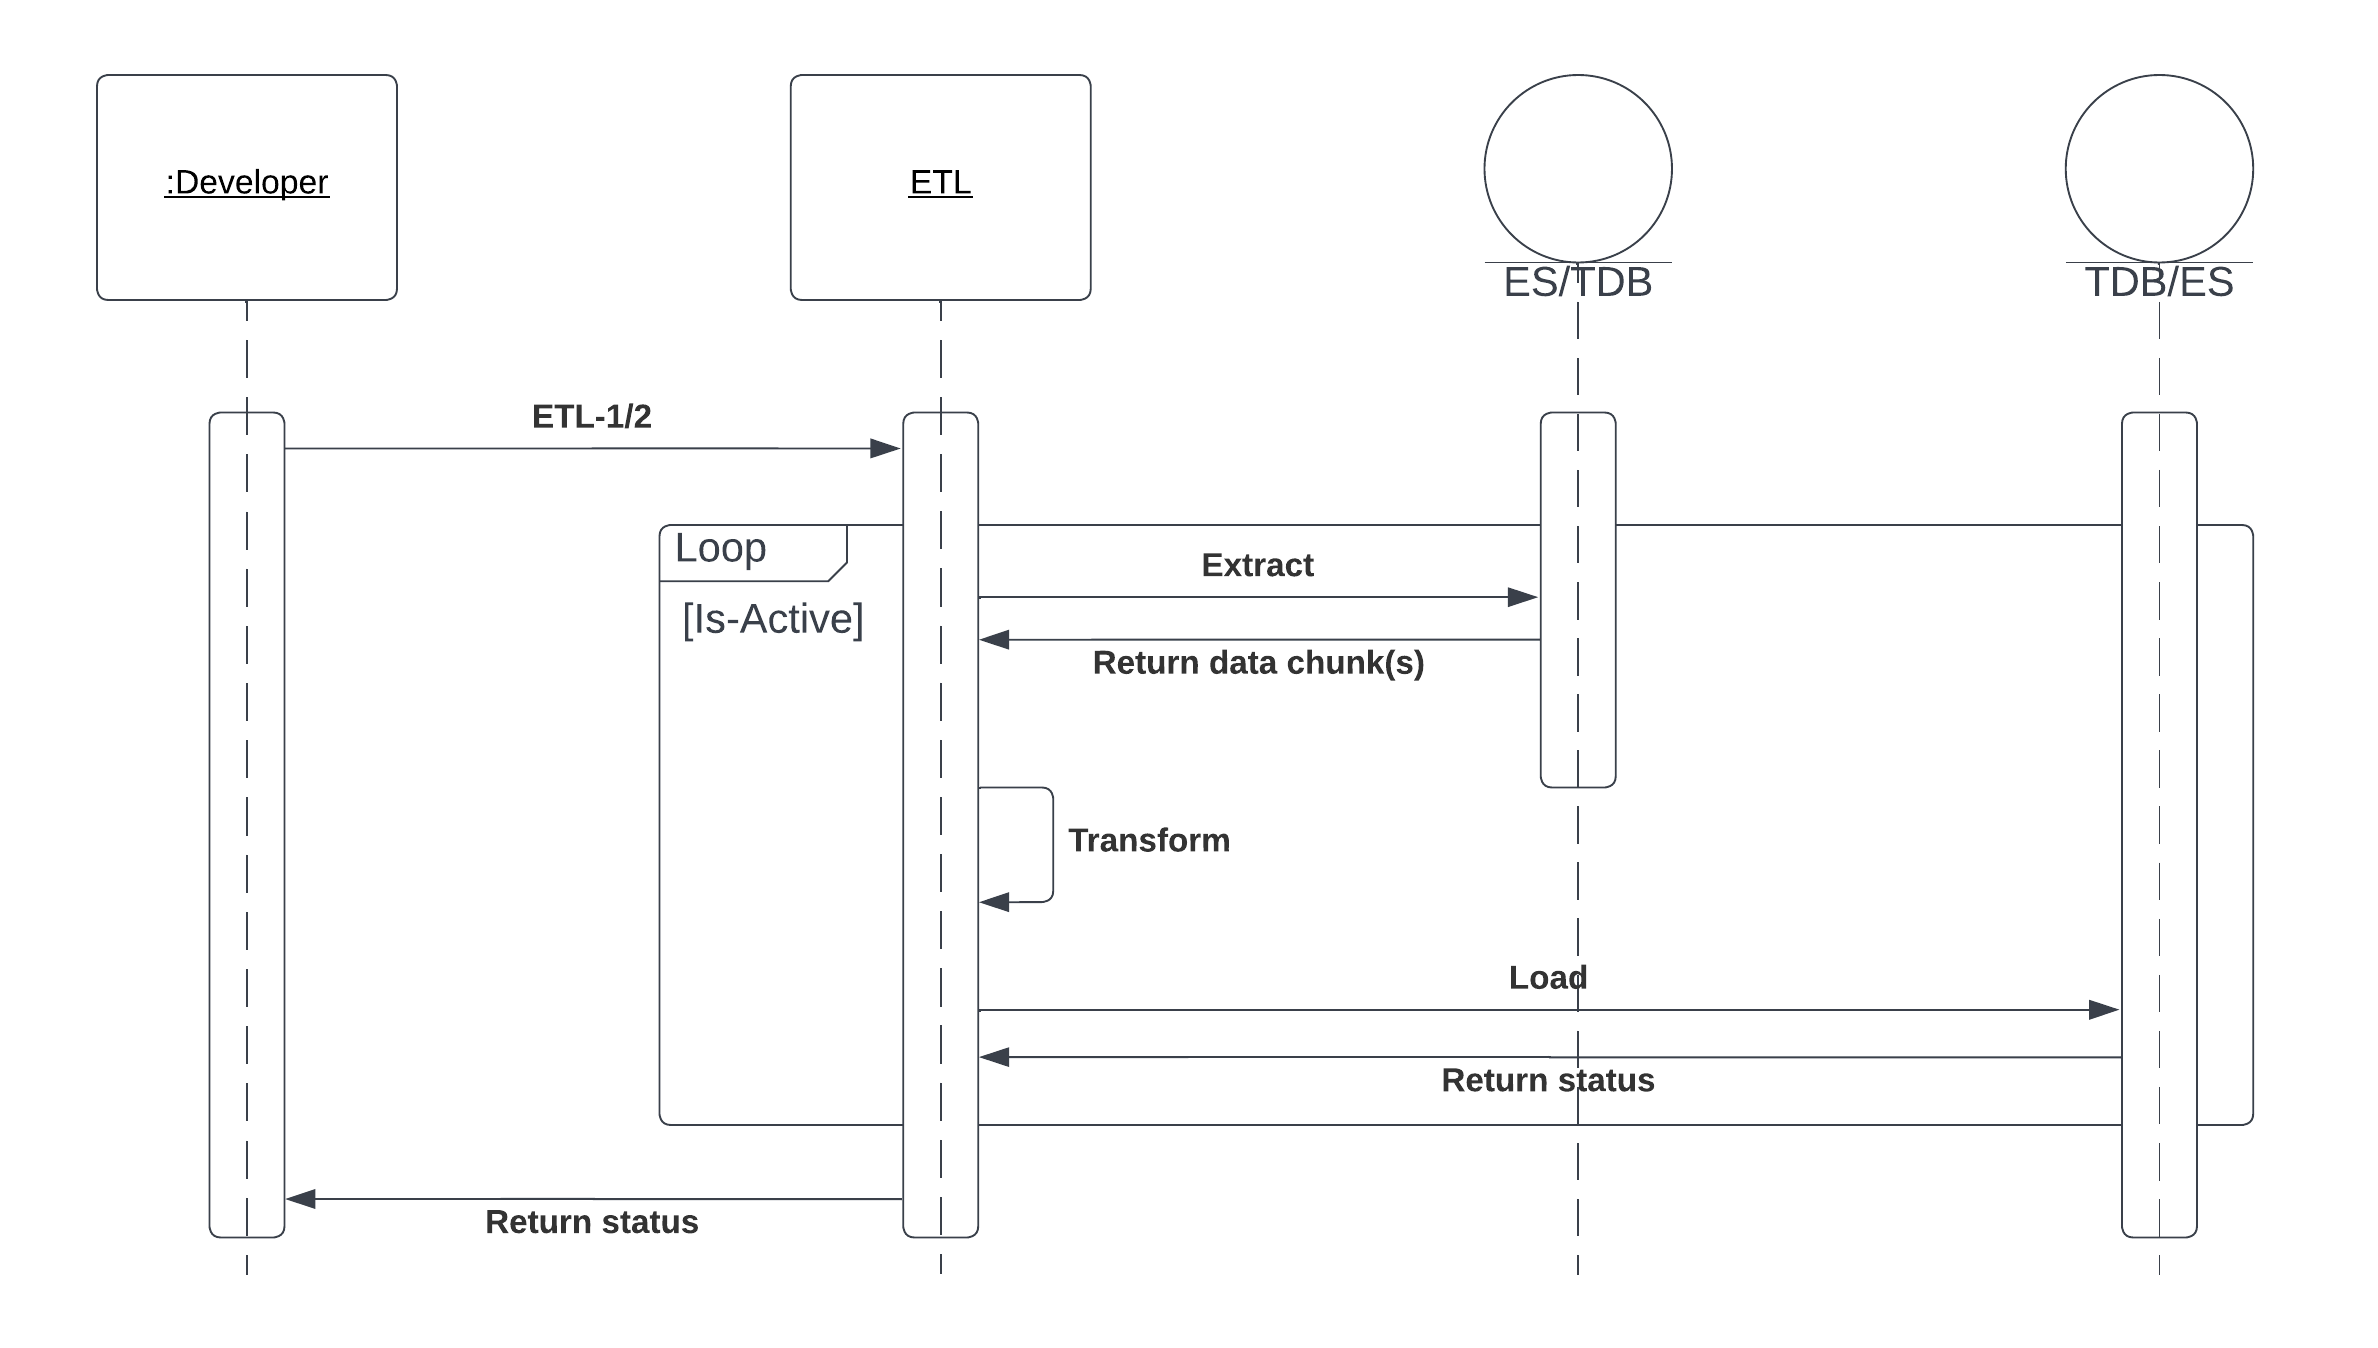
\includegraphics[width=0.95\textwidth]{../../resources/soft_sequence.png}
	\caption{Sequence diagram}
	\label{fig:soft_sequence}
\end{figure}

\paragraph{Sequential and Parallel Architecture.}
While developing the software to automate knowledge acquisition processes, we can also think of 
two main types of processing known as \textit{sequential} and \textit{parallel processing}. Writing 
a program in a sequential manner can be easy compared to the parallel one, however, there is a trade-off 
between the two. While sequentially running programs may usually be easier and faster to write, 
they may also become slower in execution time compared to that of parallel programs. Of course, this 
applies to programs that consists of many independent computations. The process of knowledge 
acquisition, in our case, contains many such computations as well. So, it is probably worth thinking 
about the software design from this aspect of processing too.
In addition to this, the real database of the company may contain millions, if not more, 
documents/products and to be able process all the database would potentially become intractable if 
executed sequentially. Parallelization with the right type of architecture and design could be 
very beneficial and improve the run-time quality several magnitudes of the order 10 or more depending 
on the machine specifications.

\begin{figure}[H]
	\centering
	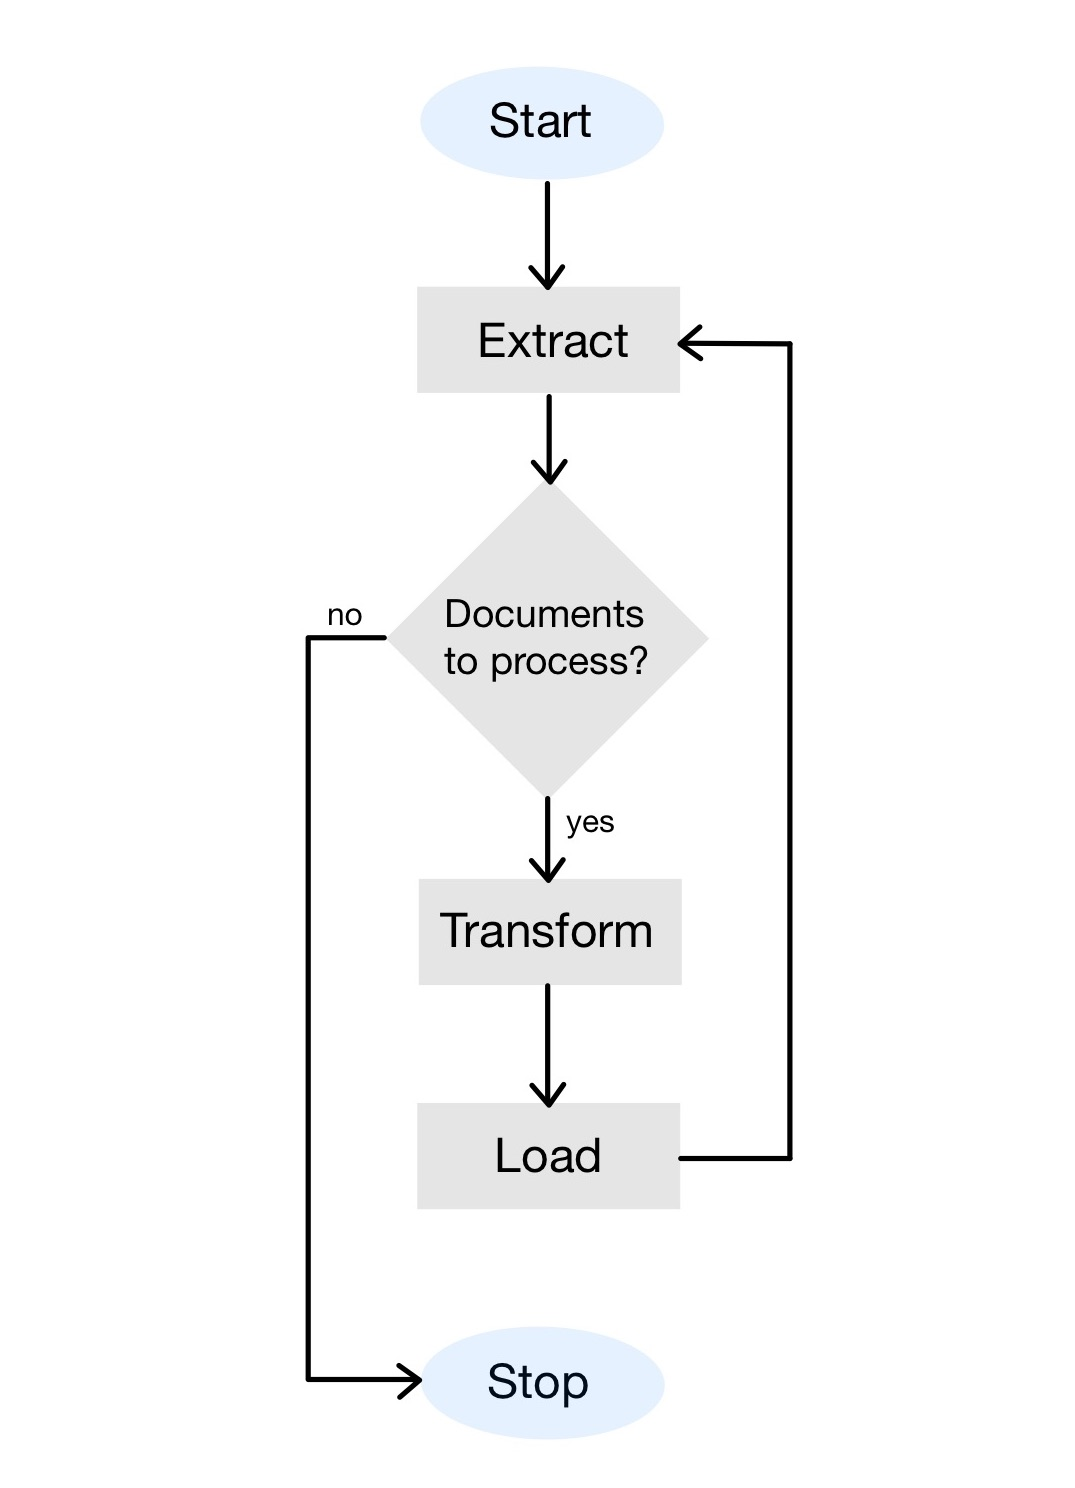
\includegraphics[width=0.55\textwidth]{../../resources/sequential_proc_arch.jpg}
	\caption{Sequential architecture}
	\label{fig:seq_arch}
\end{figure}

Figure \ref{fig:seq_arch} illustrate a simple sequential processing architecture that, by default, 
is selected when using the developed software. What this architecture tells us is that we run each 
subprocess (i.e., \textit{extract}, \textit{transform} and \textit{load}) once per a chunk of data or 
documents. Note that they may be invoked more than once within the scope of the whole process and 
this is due to the reason that the company's database may contain hundreds of GBs, if not thousands, 
all of which cannot be loaded at once to the local machine or any other ``regular'' computer that executes 
the program. For this reason, the documents or the data are extracted, transformed, and loaded in 
as many chunks as needed. If one iteration of ETL can only deal with 1000 documents and there are 
$10^9$ 
documents in the database, a million ETL processes are going to be executed one after another, in a 
sequential manner, in order to acquire 100\% of the knowledge completely.

\begin{figure}[H]
	\centering
	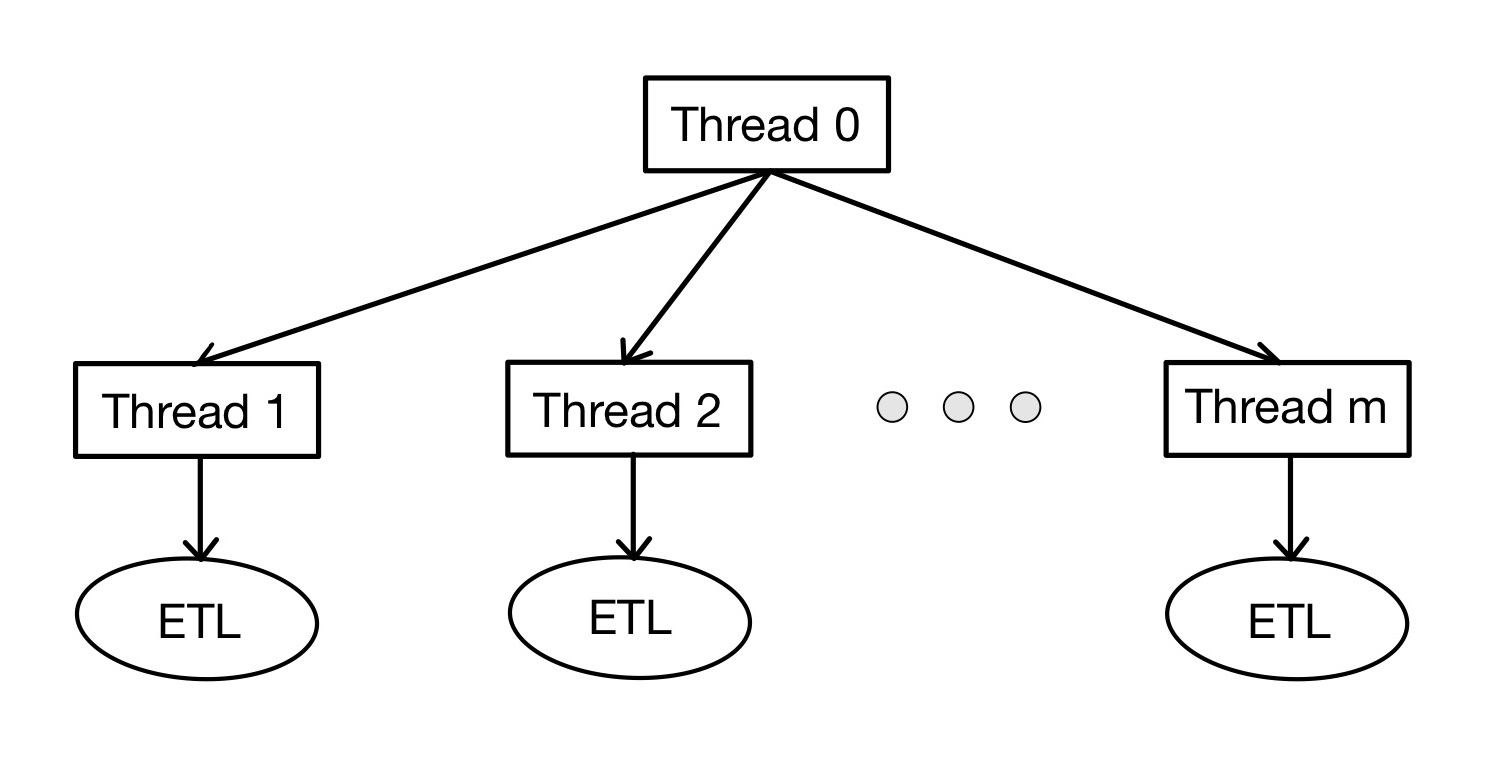
\includegraphics[width=0.75\textwidth]{../../resources/parallel_proc_arch.jpg}
	\caption{Parallel architecture}
	\label{fig:par_arch}
\end{figure}

In contrast to the sequential processing, it is also possible for one to separate ETL process to not 
wait for the other since they are completely independent. Realization of this simple fact leads us to 
develop a simple, yet faster-running, parallel processing architecture shown in figure 
\ref{fig:par_arch}.

\begin{figure}[H]
	\centering
	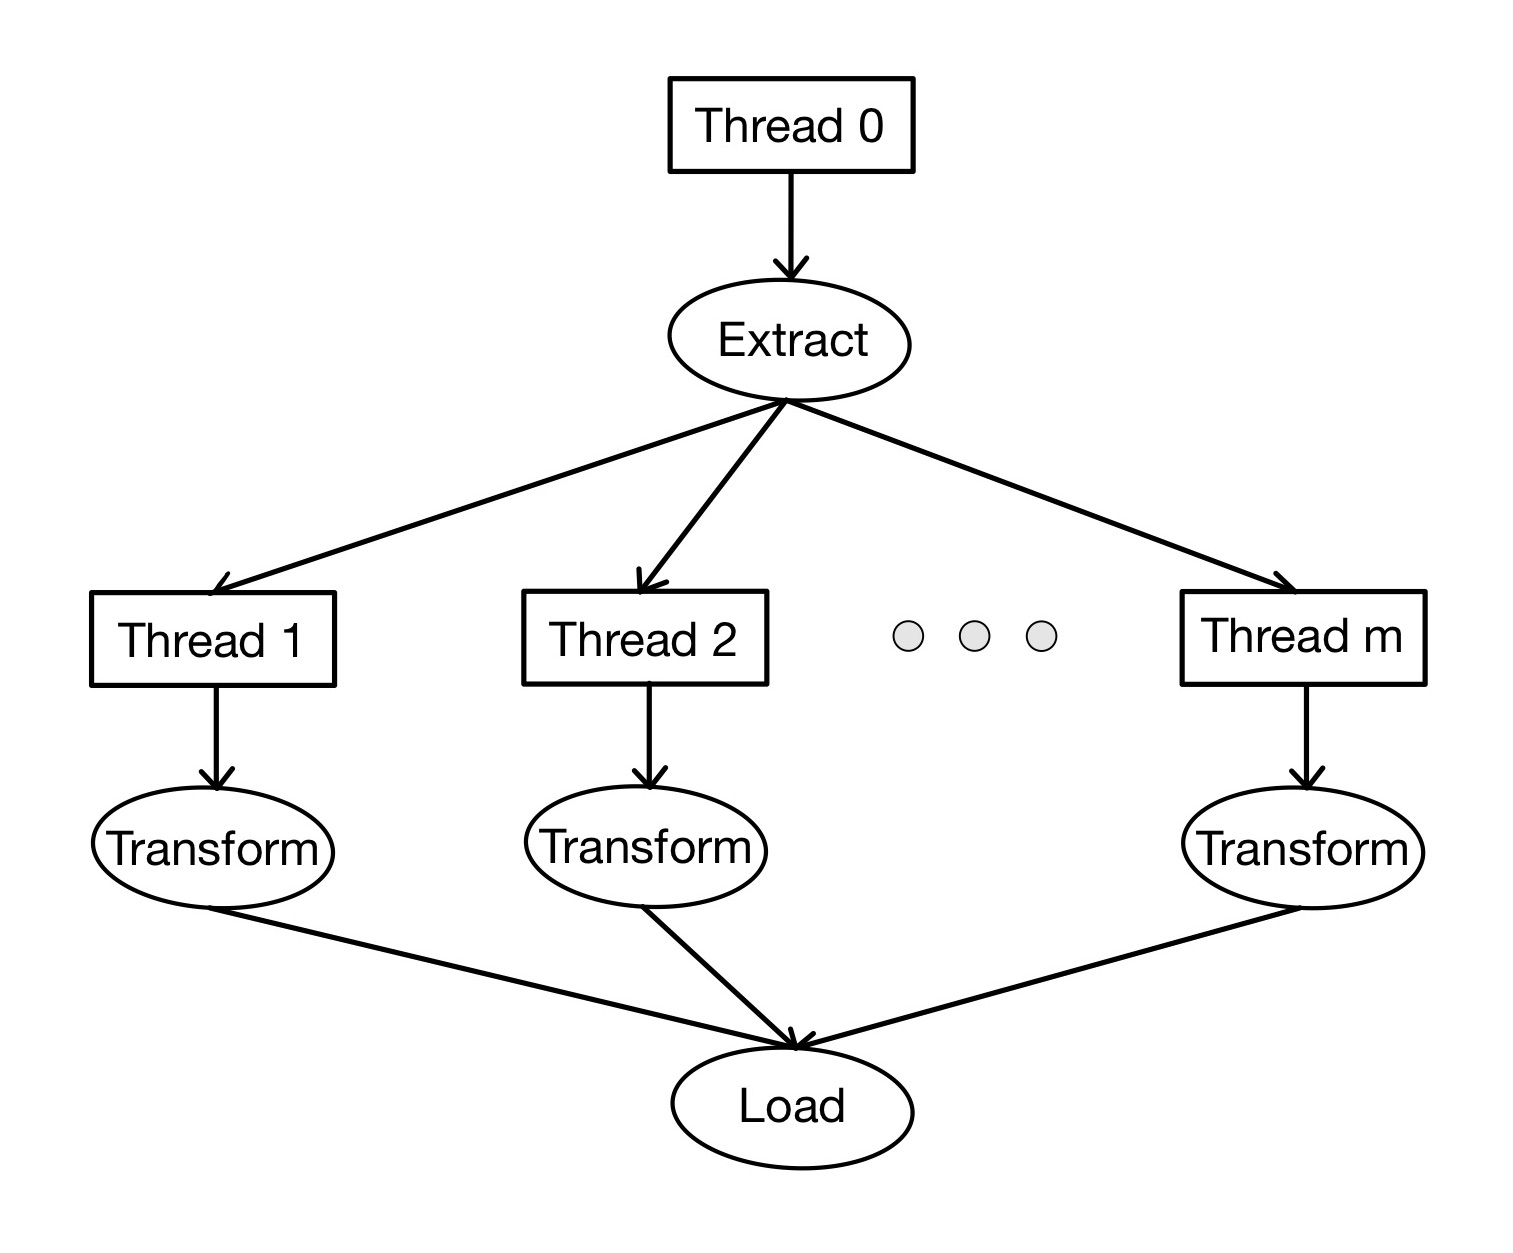
\includegraphics[width=0.75\textwidth]{../../resources/parallel_proc_arch2.jpg}
	\caption{Improved parallel architecture}
	\label{fig:par_arch2}
\end{figure}

Enhanced version of the architecture illustrated in figure \ref{fig:par_arch} can be easily realized 
if we excluded \textit{extract} and \textit{load} operations from running in a parallel fashion and 
only 
kept the \textit{transform} operation. The idea behind this architecture shown in figure 
\ref{fig:par_arch2} is the fact that each extraction and loading operation requires sending/receiving 
requests from/to a database running on some external network. It may be time-consuming to send and 
receive packets through the network when these operations are repeated many times. This is the reason, 
we can also improve the first parallel architecture by bringing the parallelism only to the 
\textit{transformation layer}. Therefore, instead of many extract-transform-load operations, we perform 
mass extraction then transformation of the vast amount of fetched documents in parallel, and finally, 
mass loading into another database.

\subsection{Specification and Implementation}

In this section, the developed software is described in terms of core implementational details that 
help to visualize and understand the underlying working principles of the carried operations. Mainly, 
there are several (sub)processes that have been described:

\begin{enumerate}
	\item Extract-Transform-Load pipeline execution
	\item Extraction process
	\item Transformation process
	\item Loading process
\end{enumerate}

The subprocesses(i.e., Extraction, Transformation and Loading) are first described in terms of 
their roles in the whole pipeline, and then the following sections break down these components by 
providing pseudo-codes and additional comments.

\paragraph{ETL Pipeline.}
\textit{ETL pipeline} is a sequence of \textbf{ETL Operations} that are executed in the given order. 
The existence of such a pipeline is for better modularity and readability. Components can easily be 
added, modified or removed from the pipeline. There are three ETL Operations or pipeline components 
that can be 
added to the ETL pipeline: \textit{Extractor}, \textit{Transformer} and \textit{Loader}. Figure 
\ref{fig:etl_pipeline} illustrates an example pipeline with these components and \textbf{*} sign on 
the top right side of each component indicates that there can be 0 or more such operations. The order 
of the components can also be arbitrary, however, it defines the processing order accordingly and 
therefore, depends on the use case of a user. Despite that, the common order of components in the 
pipeline is as shown below. Each operation takes in an input and returns an output of \textbf{Data} 
type. This constraint on the pipeline components is very helpful to build robustness and modularity.

\begin{figure}[H]
	\centering
	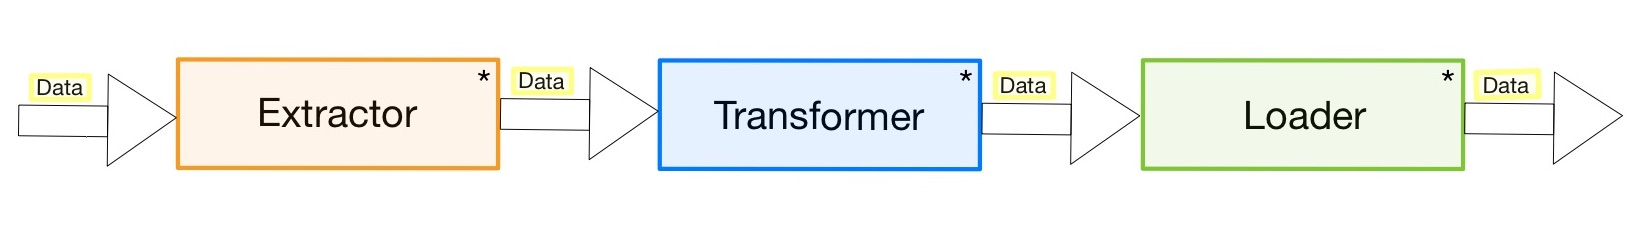
\includegraphics[width=\textwidth]{../../resources/etl_pipeline.jpg}
	\caption{ETL pipeline}
	\label{fig:etl_pipeline}
\end{figure}

The \textbf{Data} type is a simple class that has been created to serve as a unified data storage. 
By doing so, we can have restrictions, constraints and processes to check the validity of the data, 
if needed. Table \ref{tab:class_attr_data} shows the attributes and methods of this class.

\begin{table}[H]
	\centering
	\begin{tabular}{|p{0.5\textwidth}|p{0.5\textwidth}|}
		\hline
		\textbf{Attribute} & \textbf{Description} \\
		\hline
		data & Can be used to hold any type of data, however, the recommended format is the dictionary \\
		\hline
		\hline
		\textbf{Method} & \textbf{Description} \\
		\hline
		- & - \\
		\hline
	\end{tabular}
	\caption{Data Class Attributes/Methods}
	\label{tab:class_attr_data}
\end{table}

There are two different ETL pipelines used for the knowledge acquisition named as \textit{ETL-1} and 
\textit{ETL-2}. ETL-1 is to build and store a knowledge graph (KG) in a TDB database by fetching the raw 
documents from the original ES database. ETL-2 is to build a semantic ES (S-ES) database by using the 
already existing KG and make the documents searchable in a more semantic manner. For the detailed 
explaination of how the pipeline works, I am going to give demonstrative examples for both ETL pipelines 
and describe them step-by-step.

ETL-1 pipeline contains \textbf{ESQuery} as an \textit{extractor}, \textbf{ES2TDB} as a 
\textit{transformer} and \textbf{TerminalOps} as a \textit{loader}. The execution of this pipeline 
yields KG built upon the documents stored the original ES database. First, ESQuery 
fetches the documents chunk-by-chunk with the given document count per chunk and the total chunk count. 
Figure \ref{fig:es_doc_example} illustrates an example row of the ES database. Fetched documents are 
transformed by ES2TDB into OTTR instances as shown in figure \ref{fig:ottr_instance_example}.
This KG is then stored in a Jena's TDB database by the TerminalOps. Some of the final RDF/Turtle 
triples represented in the store KG are illustrated by figure \ref{fig:rdf_ttl_example} (see 
figure \ref{fig:rdf_ttl_example_full} for the full version). ETL-1 takes a relational ES database of 
the company as its input and builds a second Jena Fuseki (TDB) database which contains the KG.

% \begin{figure}[H]
% \centering
% \begin{subfigure}{\linewidth}
% 	\centering
% 
% 	\begin{table}[H]
% 		\begin{tabular}{|p{0.20\linewidth}|p{0.20\linewidth}|p{0.25\linewidth}|p{0.25\linewidth}|}
% 			\hline
% 			\textbf{PartFamily} & \textbf{PartNumber} & \textbf{PartFamilyName} & \textbf{PartNumberName} \\
% 			\hline
% 			90-22112018-056525 & LC1BL34U31 & [en] TeSys B contactor 4P 800A 240V AC - LC1BL34U31 & [en] TeSys B contactor 4P 800A 240V AC - LC1BL34U31 \\
% 			\hline
% 		\end{tabular}
% 	\end{table}
% 
% 	\caption{Document fetched from the ES database}
% 	\label{fig:es_doc_example}
% \end{subfigure}
% \end{figure}

% \begin{figure}[H]
% \ContinuedFloat
% 
% \begin{subfigure}{\textwidth}
%   \centering
% 
%   \begin{table}[H]
% 	  \begin{tabular}{|p{0.98\linewidth}|}
% 		  \hline
% 		  tp:createPartNumberInstance(tp:PNLC1BL34U31, tp:IDLC1BL34U31, tp:PF90-22112018-056525, tp:Text-6378022537900392513). \\
% 		  tp:createPartFamilyInstance(tp:PF90-22112018-056525, tp:ID90-22112018-056525, tp:Text-2992260873777870348). \\
% 		  tp:createTextInstance(tp:Text-6378022537900392513, "TeSys B contactor 4P 800A 240V AC"^^xsd:string, tp:Language-def, (tp:ID4P,tp:ID800A,tp:ID240V)). \\
% 		  tp:createTextInstance(tp:Text-2992260873777870348, "TeSys B contactor 4P 800A 240V AC - LC1BL34U31"^^xsd:string, tp:Language-def, (tp:ID4P,tp:ID800A,tp:ID240V,tp:IDLC1BL34U31)). \\
% 		  tp:createIdInstance(tp:IDLC1BL34U31, "LC1BL34U31"^^xsd:string). \\
% 		  tp:createIdInstance(tp:ID90-22112018-056525, "90-22112018-056525"^^xsd:string). \\
% 		  tp:createIdInstance(tp:ID4P, "4P"^^xsd:string). \\
% 		  tp:createIdInstance(tp:ID800A, "800A"^^xsd:string). \\
% 		  tp:createIdInstance(tp:ID240V, "240V"^^xsd:string). \\
% 		  \hline
% 	  \end{tabular}
%   \end{table}
% 
%   \caption{OTTR instance}
%   \label{fig:ottr_instance_example}
% \end{subfigure}
% \end{figure}

% \begin{figure}[H]
% \ContinuedFloat
% 
% \begin{subfigure}{\textwidth}
%   \centering
% 
%   \begin{table}[H]
% 	  \begin{tabular}{|p{0.31\linewidth}|p{0.31\linewidth}|p{0.31\linewidth}|}
% 		  \hline
% 		  \textbf{Subject} & \textbf{Predicate} & \textbf{Object} \\
% 		  \hline
% 		  \multirow{4}{*}{tp:PNLC1BL34U31} & rdf:type & tp:PartNumber \\
% 		   & gist:isIdentifiedBy & tp:IDLC1BL34U31 \\
% 		   & gist:isDescribedIn & tp:Text-6378022537900392513 \\
% 		   & tp:hasPartFamily & tp:PF90-22112018-056525 \\
% 		  \hline
% 		  \multirow{3}{*}{tp:PF90-22112018-056525} & rdf:type & tp:PartFamily \\
% 		   & gist:isIdentifiedBy & tp:ID90-22112018-056525 \\
% 		   & gist:isDescribedIn & tp:Text-2992260873777870348 \\
% 		  \hline
% 		  \multirow{3}{*}{tp:Text-6378022537900392513} & rdf:type & gist:Text \\
% 		   & gist:containedText & "TeSys B contactor 4P 800A 240V AC - LC1BL34U31" \\
% 		   & gist:isExpressedIn & tp:Language-def \\
% 		  \hline
% 		  \multirow{3}{*}{tp:IDLC1BL34U31} & rdf:type & gist:ID \\
% 		   & gist:uniqueText & "LC1BL34U31" \\
% 		   & gist:isPartOf & tp:Text-6378022537900392513 \\
% 		  \hline
% 	  \end{tabular}
%   \end{table}
% 
%   \caption{RDF/Turtle triples}
%   \label{fig:rdf_ttl_example}
% \end{subfigure}
% \caption{ETL from ES to TDB example}
% \label{fig:etl-1_example}
% \end{figure}

ETL-2 pipeline contains \textbf{SPARQLQuery} as an \textit{extractor}, \textbf{TDB2ES} as a 
\textit{transformer} and \textbf{JSONOps} as a \textit{loader}. This pipeline is executed after the 
execution of the first one and therefore, the existence of the KG as the single source of truth is 
already 
guaranteed. The necessary instances from the KG stored in the TDB database are fetched through one or 
more SPARQL queries as shown in figures \ref{fig:tdb_sparql_example} and 
\ref{fig:tdb_response_example}\footnote{tp = $<$https://ontologies.traceparts.com/$>$} 
\footnote{gist = $<$https://ontologies.semanticarts.com/gist/$>$} 
\footnote{rdf = $<$http://www.w3.org/1999/02/22-rdf-syntax-ns\#$>$}. Obtained responses are 
transformed to a suitable dictionary format according to the already-specified schema of the 
S-ES database. After the transformation of the fetched instances, the prepared Python dictionary 
is dumped to a JSON file as the result of the JSONOps execution. 
Figure \ref{fig:ses_json_example} illustrates the transformed version of the entities in a JSON format.
ETL-2 takes the KG stored in the Jena Fuseki (TDB) database as its input and builds a third ES 
database with some additional semantics.

\begin{figure}[H]
\centering
\begin{subfigure}{\linewidth}
	\centering

	\begin{table}[H]
		\begin{tabular}{|p{0.20\linewidth}|p{0.20\linewidth}|p{0.25\linewidth}|p{0.25\linewidth}|}
			\hline
			\textbf{PartFamily} & \textbf{PartNumber} & \textbf{PartFamilyName} & \textbf{PartNumberName} \\
			\hline
			90-22112018-056525 & LC1BL34U31 & [en] TeSys B contactor 4P 800A 240V AC - LC1BL34U31 & [en] TeSys B contactor 4P 800A 240V AC - LC1BL34U31 \\
			\hline
		\end{tabular}
	\end{table}

	\caption{Document fetched from the ES database}
	\label{fig:es_doc_example}
\end{subfigure}
\end{figure}

\begin{figure}[H]
\ContinuedFloat

\begin{subfigure}{\textwidth}
  \centering

  \begin{table}[H]
	  \begin{tabular}{|p{0.98\linewidth}|}
		  \hline
		  tp:createPartNumberInstance(tp:PNLC1BL34U31, tp:IDLC1BL34U31, tp:PF90-22112018-056525, tp:Text-6378022537900392513). \\
		  tp:createPartFamilyInstance(tp:PF90-22112018-056525, tp:ID90-22112018-056525, tp:Text-2992260873777870348). \\
		  tp:createTextInstance(tp:Text-6378022537900392513, "TeSys B contactor 4P 800A 240V AC"\^{}\^{}xsd:string, tp:Language-def, (tp:ID4P,tp:ID800A,tp:ID240V)). \\
		  tp:createTextInstance(tp:Text-2992260873777870348, "TeSys B contactor 4P 800A 240V AC - LC1BL34U31"\^{}\^{}xsd:string, tp:Language-def, (tp:ID4P,tp:ID800A,tp:ID240V,tp:IDLC1BL34U31)). \\
		  tp:createIdInstance(tp:IDLC1BL34U31, "LC1BL34U31"\^{}\^{}xsd:string). \\
		  tp:createIdInstance(tp:ID90-22112018-056525, "90-22112018-056525"\^{}\^{}xsd:string). \\
		  tp:createIdInstance(tp:ID4P, "4P"\^{}\^{}xsd:string). \\
		  tp:createIdInstance(tp:ID800A, "800A"\^{}\^{}xsd:string). \\
		  tp:createIdInstance(tp:ID240V, "240V"\^{}\^{}xsd:string). \\
		  \hline
	  \end{tabular}
  \end{table}

  \caption{OTTR instance}
  \label{fig:ottr_instance_example}
\end{subfigure}
% \end{figure}
% 
% \begin{figure}[H]
% \ContinuedFloat

\begin{subfigure}{\textwidth}
  \centering

  \begin{table}[H]
	  \begin{tabular}{|p{0.31\linewidth}|p{0.25\linewidth}|p{0.38\linewidth}|}
		  \hline
		  \textbf{Subject} & \textbf{Predicate} & \textbf{Object} \\
		  \hline
		  \multirow{4}{*}{tp:PNLC1BL34U31} & rdf:type & tp:PartNumber \\
		   & gist:isIdentifiedBy & tp:IDLC1BL34U31 \\
		   & gist:isDescribedIn & tp:Text-6378022537900392513 \\
		   & tp:hasPartFamily & tp:PF90-22112018-056525 \\
		  \hline
		  \multirow{3}{*}{tp:PF90-22112018-056525} & rdf:type & tp:PartFamily \\
		   & gist:isIdentifiedBy & tp:ID90-22112018-056525 \\
		   & gist:isDescribedIn & tp:Text-2992260873777870348 \\
		  \hline
		  \multirow{3}{*}{tp:Text-6378022537900392513} & rdf:type & gist:Text \\
		   & gist:containedText & "TeSys B contactor 4P 800A 240V AC - LC1BL34U31" \\
		   & gist:isExpressedIn & tp:Language-def \\
		  \hline
		  \multirow{3}{*}{tp:IDLC1BL34U31} & rdf:type & gist:ID \\
		   & gist:uniqueText & "LC1BL34U31" \\
		   & gist:isPartOf & tp:Text-6378022537900392513 \\
		  \hline
	  \end{tabular}
  \end{table}

  \caption{RDF/Turtle triples}
  \label{fig:rdf_ttl_example}
\end{subfigure}
\caption{ETL from ES to TDB example}
\label{fig:etl-1_example}
\end{figure}

\newpage
\begin{figure}[H]
\centering

\begin{subfigure}{\linewidth}
	\centering

	\begin{lstlisting}
	select ?subject ?predicate ?object
	where {
	  ?subject ?predicate ?object
	}
	limit 5
	offset 0
	\end{lstlisting}

	\caption{SPARQL query}
	\label{fig:tdb_sparql_example}
\end{subfigure}
% \end{figure}
% 
% \begin{figure}[H]
% \ContinuedFloat

\begin{subfigure}{\textwidth}
  \centering

  \begin{table}[H]
	  \begin{tabular}{|p{0.35\linewidth}|p{0.30\linewidth}|p{0.31\linewidth}|}
		  \hline
		  \textbf{Subject} & \textbf{Predicate} & \textbf{Object} \\
		  \hline
		  tp:ID10-12032019-066017 & rdf:type & gist:ID \\
		  tp:ID10-12032019-066017 & gist:uniqueText & "10-12032019-066017" \\
		  tp:IDZB5FA46C0 & rdf:type & gist:ID \\
		  tp:IDZB5FA46C0 & gist:uniqueText & "ZB5FA46C0" \\
		  tp:Text79763625448103550 & rdf:type & gist:Text \\
		  \hline
	  \end{tabular}
  \end{table}

  \caption{SPARQL response (KG)}
  \label{fig:tdb_response_example}
\end{subfigure}
\end{figure}

\begin{figure}[H]
\ContinuedFloat

\begin{subfigure}{\textwidth}
  \centering

  \begin{table}[H]
	  \begin{tabular}{|p{0.20\linewidth}|p{0.75\linewidth}|}
		  \hline
		  \textbf{Key} & \textbf{Value} \\
		  \hline
		  doc\_id & 90-22112018-056525:LC1BL34Q31 \\
		  \hline
		  uri & https://ontologies.traceparts.com/PF90-22112018-056525 \\
		  \hline
		  \multirow{4}{*}{concept\_uris} & tp:ID4P \\
		   & tp:IDLC1BL34Q31 \\
		   & tp:ID800A \\
		   & tp:ID240V \\
		  \hline
		  \multirow{2}{*}{searcable\_texts} & def: TeSys B contactor 4P 800A 240V AC - LC1BL34Q31 \\ 
		   & en: TeSys B contactor 4P 800A 240V AC - LC1BL34Q31 \\
		  \hline
	  \end{tabular}
  \end{table}

  \caption{RDF/Turtle triple}
  \label{fig:ses_json_example}
\end{subfigure}
\caption{ETL from TDB to ES example}
\label{fig:etl-2_example}
\end{figure}

\textit{ETL} algorithm shown in \ref{alg:etl} executes each pipeline component(i.e., extractor, 
transformer and loader) in the given order. If a user provides \{``parallelism'': 0\} in the data 
object to be given to \textit{run} method of the ETL object, the components are executed in a 
sequential fashion, one by one. Otherwise, the transformation operation is executed in a parallel 
fashion.

\begin{algorithm}[H]
\caption{ETL}\label{alg:etl}
\begin{algorithmic}
\Require \texttt{OperationalData}
\Ensure \texttt{OperationalData}

\While{\texttt{the process should not terminate}}
\If{\texttt{sequential run}}
	\For{\texttt{component in pipeline}}
		\State \texttt{data} = \texttt{component}.\texttt{run}(\texttt{data})
	\EndFor
\Else 	\Comment{for parallel run}
	\State \texttt{get extractor, transformer, loader from the pipeline}
	\State \texttt{extractor.run}(\texttt{data})
	\State \texttt{allocate $m$ buffers inside data object}
	\State \texttt{allocate $m$ threads to run transformer on the respective buffer}

	\For{\texttt{thread in threads}}
	\State \texttt{thread.run()}	\Comment{Each thread performs transformations on a subset of documents and stores the result temporarility on the corresponding index in buffer}
	\EndFor

	\State \texttt{wait for all $m$ threads to finish}
	\State \texttt{data} = \texttt{loader}.\texttt{run}(\texttt{data})
\EndIf
\EndWhile
\end{algorithmic}
\end{algorithm}

The \textit{pipeline} attribute of an ETL object can be initialized with an arbitrary number of 
ETL operations and in an arbitrary order. Such an arbitrary pipeline would work just fine if executed  
sequentially. Parallelized execution is only suitable for this project since there is only one of 
each operation per the whole ETL process. If the pipeline was to contain several extractors/loaders 
then a more generic implementation would be required to optimize it.

\paragraph{Extractor.}
The Extractor class is a process-only class\footnote{By process-only class, I mean a class that 
consists of only methods and not attributes since the whole purpose of using them is mostly 
processing the given data and returning the modified version of it back.}. Table 
\ref{tab:class_attr_extractor} shows the attributes and methods of the Extractor class. There are 
no attributes and only two abstract methods one of which(i.e., \texttt{run(\ldots)}) is inheretied 
from the parent class ETLOperation.

\begin{table}[H]
	\centering
	\begin{tabular}{|p{0.5\textwidth}|p{0.5\textwidth}|}
		\hline
		\textbf{Attribute} & \textbf{Description} \\ 
		- & - \\
		\hline
		\hline
		\textbf{Method} & \textbf{Description} \\ 
		\hline
		extract(data: OperationalData) $\rightarrow$ OperationalData & abstract \\
		\hline
		run(data: OperationalData) $\rightarrow$ OperationalData & abstract, inherited \\
		\hline
	\end{tabular}
	\caption{Extractor Class Attributes/Methods}
	\label{tab:class_attr_extractor}
\end{table}

\begin{algorithm}
\caption{ESQuery/SPARQLQuery-Extractor}\label{alg:etl_extractor}
\begin{algorithmic}
\Require requestBody, method, url, numChunk
\Ensure docs (as a list of numChunk chunks)

\State session = createSession()	\Comment{created once within an object}
\If{scrollRequest}	\Comment{getting response partially}
	\State requestBody = buildScrollQuery()	\Comment{different implementation for different databases}
\EndIf
% \algstore{myalgextractor}
% \end{algorithmic}
% \end{algorithm}
% 
% \begin{algorithm}
% \begin{algorithmic}
% \algrestore{myalgextractor}
\State response = session.request(requestBody, method, url)
\State extract \textbf{header} and \textbf{hits} from \textbf{response}
\State chunks = []	\Comment{initialize chunks as an empty list}
\State chunkSize = len(hits) / numChunk

\For{$i$ in $\{0, \cdots, \text{numChunk}-1\}$}
	\State chunks.append(hits[$i*\text{chunkSize}$ : $(i+1)*\text{chunkSize}$)	\Comment{add sublist of documents}
\EndFor
\State chunks.append(hits[$(\text{numChunk}-1)*\text{chunkSize}$ : ])	\Comment{add the residual documents, if any}

\State \Return header, chunks
\end{algorithmic}
\end{algorithm}

% \begin{algorithm}[H]
% \caption{ESQuery/SPARQLQuery-Extractor}\label{alg:etl_extractor}
% \begin{algorithmic}
% \Require requestBody, method, url, numChunk
% \Ensure docs (as a list of numChunk chunks)
% 
% \State session = createSession()	\Comment{created once within an object}
% \If{scrollRequest}	\Comment{getting response partially}
% 	\State requestBody = buildScrollQuery()	\Comment{different implementation for different databases}
% \EndIf
% 
% \State response = session.request(requestBody, method, url)
% \State extract \textbf{header} and \textbf{hits} from \textbf{response}
% \State chunks = []	\Comment{initialize chunks as an empty list}
% \State chunkSize = len(hits) / numChunk
% 
% \For{$i$ in $\{0, \cdots, \text{numChunk}-1\}$}
% 	\State chunks.append(hits[$i*\text{chunkSize}$ : $(i+1)*\text{chunkSize}$)	\Comment{add sublist of documents}
% \EndFor
% \State chunks.append(hits[$(\text{numChunk}-1)*\text{chunkSize}$ : ])	\Comment{add the residual documents, if any}
% 
% \State \Return header, chunks
% \end{algorithmic}
% \end{algorithm}

Algorithm \ref{alg:etl_extractor} illustrates how the specific extraction processes from ElasticSearch 
(ESQuery) and TDB(SPARQLQuery) are performed. The only important difference between these processes is 
in the query-building part. Scroll queries are known as queries performed on the databases resulting 
in 
partial responses. When the response may be too huge in size, we request only a part of it iteratively 
until we reach to the end of it and this is the main reason why scroll queries are very useful. More 
specifically, the scroll queries for the request body are built differently for ES and TDB endpoints. For 
example, building a scroll query requires a \textit{scroll ID} of the last query in the ES database while there 
is an offset value set by the user to get the next piece of partial response in the TDB database. 
So, the implementation of building scroll queries has solely built upon scroll IDs and offset values 
for the respective endpoints.

\paragraph{Transformer.}
Transformer is a pure abstract class which is used to define an interface for different 
transformation implementations. Table \ref{tab:class_attr_transformer} illustrates the 
attributes and methods of this class.

\begin{table}[H]
	\centering
	\begin{tabular}{|p{0.5\textwidth}|p{0.5\textwidth}|}
		\hline
		\textbf{Attribute} & \textbf{Description} \\ 
		nlp & spacy.language.Language \\
		\hline
		\hline
		\textbf{Method} & \textbf{Description} \\ 
		\hline
		transform(data: OperationalData) $\rightarrow$ OperationalData & abstract \\
		\hline
		run(data: OperationalData) $\rightarrow$ OperationalData & abstract, inherited \\
		\hline
	\end{tabular}
	\caption{Transformer Class Attributes/Methods}
	\label{tab:class_attr_transformer}
\end{table}

Algorithms \ref{alg:etl_transformer_es2tdb} and \ref{alg:etl_transformer_tdb2es} illustrate how 
the specific transformation processes are executed to transform entites coming from ES(original 
database) to TDB(knowledge graph storage) and from TDB(knowledge graph storage) to ES(semantic ES 
database) respectively.

\begin{algorithm}
\caption{ES2TDB-Transformer}\label{alg:etl_transformer_es2tdb}
\begin{algorithmic}
\Require docs
\Ensure rdf/ttl file

\State file = open(filepath)
\For{doc in docs}
	\State fetch \textbf{pfID} from \textbf{doc}
	\State fetch \textbf{pnNumber} from \textbf{doc}
	\State fetch \textbf{pfNamesDict} from \textbf{doc}
	\State fetch \textbf{pnNamesDict} from \textbf{doc}

	\State file.write(processID(pfID))	\Comment{processID returns ID intialization string in OTTR format}
	\State file.write(processID(pnNumber))
\algstore{myalges2tdb}
\end{algorithmic}
\end{algorithm}

\begin{algorithm}
\begin{algorithmic}
\algrestore{myalges2tdb}
	\For{language, pfName in pfNamesDict}
	\State file.write(processPF(nlp, pfID, pfName, language)	\Comment{processPF returns PartFamily initialization string in OTTR format}
	\EndFor

	\For{language, pfName in pnNamesDict}
	\State file.write(processPN(nlp, pnNumber, pnName, language) 	\Comment{processPN returns PartNumber initialization string in OTTR format}
	\EndFor
\EndFor

\State compileOTTR(filepath)	\Comment{compilation of generated OTTR instance file(s)}
\end{algorithmic}
\end{algorithm}

% \begin{algorithm}[H]
% \caption{ES2TDB-Transformer}\label{alg:etl_transformer_es2tdb}
% \begin{algorithmic}
% \Require docs
% \Ensure rdf/ttl file
% 
% \State file = open(filepath)
% \For{doc in docs}
% 	\State fetch \textbf{pfID} from \textbf{doc}
% 	\State fetch \textbf{pnNumber} from \textbf{doc}
% 	\State fetch \textbf{pfNamesDict} from \textbf{doc}
% 	\State fetch \textbf{pnNamesDict} from \textbf{doc}
% 
% 	\State file.write(processID(pfID))	\Comment{processID returns ID intialization string in OTTR format}
% 	\State file.write(processID(pnNumber))
% 
% 	\For{language, pfName in pfNamesDict}
% 	\State file.write(processPF(nlp, pfID, pfName, language)	\Comment{processPF returns PartFamily initialization string in OTTR format}
% 	\EndFor
% 
% 	\For{language, pfName in pnNamesDict}
% 	\State file.write(processPN(nlp, pnNumber, pnName, language) 	\Comment{processPN returns PartNumber initialization string in OTTR format}
% 	\EndFor
% \EndFor
% 
% \State compileOTTR(filepath)	\Comment{compilation of generated OTTR instance file(s)}
% \end{algorithmic}
% \end{algorithm}

As shown in algorithm \ref{alg:etl_transformer_es2tdb}, the transformer \textit{ES2TDB} creates 
an empty OTTR instance file first. Each document given as the argument to this function is iterated 
one-by-one and part family number, part name number, part family description and part number 
description are gathered and appended to the instance file. However, gathering IDs for part 
families/numbers requires NLP\footnote{Natural Language Processing} to extract them from the texts. 
For this purpose, we use spaCy\footnote{https://spacy.io} library which is well-known and used 
reliably by many other companies. To extract IDs from the given text, a regular expression is used 
as a heuristic. Finally, the instance file is compiled to RDF/Turtle triples with \textit{Lutra} 
which is a compiler for OTTR language.

% \begin{algorithm}[H]
% \caption{TDB2ES-Transformer}\label{alg:etl_transformer_tdb2es}
% \begin{algorithmic}
% \Require docs, responses
% \Ensure json text
% 
% \For{response in responses}
% 	\State result = {}	\Comment{initialize empty dictionary}
% 	\State docID = response['pf\_text'] + response['pn\_text']
% 	
% 	\If{docID has not been processed already}
% 	\State docs.append(result)	\Comment{mark it as processed}
% 	\Else
% 		\State result = documentWith(docID)		\Comment{find and return the corresponding document}
% 	\EndIf
% 
% 	\State result['docID'] = docID		\Comment{the first field of final json}
% 	\State result['uri'] = response['pf\_uri']		\Comment{the second field of final json}
% 
% 	\If{result has no field named 'concept\_uris'}
% 		\State result['concept\_uris'] = []	\Comment{initialize concept uris as an empty list}
% 	\EndIf
% 
% 	\State fidURI = response['fid\_uri']	\Comment{PartFamily uri}
% 	\State nidURI = response['fid\_uri']	\Comment{PartNumber uri}
% 
% 	\If{fidURI is not in result['concept\_uris']}
% 		\State result['concept\_uris'].append(fidURI)
% 	\EndIf
% 	\If{nidURI is not in result['concept\_uris']}
% 		\State result['concept\_uris'].append(nidURI)
% 	\EndIf
% 
% 	\If{result has no field named 'searchable\_texts'}
% 		\State result['searchable\_texts] = {}	\Comment{initialize searchable texts as an empty dictionary}
% 	\EndIf
% 
% 	\State flang = response['flang\_uri']	\Comment{uri of the language of the PartFamily text/description}
% 	\State nlang = response['nlang\_uri']	\Comment{uri of the langauge of the PartNumber text/description}
% 
% 	result['searchable\_texts'][flang] = response['ftext']	\Comment{PartFamily text/description}
% 	result['searchable\_texts'][nlang] = response['ntext']	\Comment{PartNumber text/description}
% \EndFor
% \end{algorithmic}
% \end{algorithm}

\begin{algorithm}[H]
\caption{TDB2ES-Transformer}\label{alg:etl_transformer_tdb2es}
\begin{algorithmic}                   % enter the algorithmic environment
\Require docs, responses
\Ensure json text

\For{response in responses}
	\State result = {}	\Comment{initialize empty dictionary}
	\State docID = response['pf\_text'] + response['pn\_text']
	
	\If{docID has not been processed already}
	\State docs.append(result)	\Comment{mark it as processed}
	\Else
		\State result = documentWith(docID)		\Comment{find and return the corresponding document}
	\EndIf

\algstore{myalgtdb2es}
\end{algorithmic}
\end{algorithm}

\begin{algorithm}[H]
\begin{algorithmic}                   % enter the algorithmic environment
\algrestore{myalgtdb2es}
	\State result['docID'] = docID		\Comment{the first field of final json}
	\State result['uri'] = response['pf\_uri']		\Comment{the second field of final json}

	\If{result has no field named 'concept\_uris'}
		\State result['concept\_uris'] = []	\Comment{initialize concept uris as an empty list}
	\EndIf

	\State fidURI = response['fid\_uri']	\Comment{PartFamily uri}
	\State nidURI = response['fid\_uri']	\Comment{PartNumber uri}

	\If{fidURI is not in result['concept\_uris']}
		\State result['concept\_uris'].append(fidURI)
	\EndIf
	\If{nidURI is not in result['concept\_uris']}
		\State result['concept\_uris'].append(nidURI)
	\EndIf

	\If{result has no field named 'searchable\_texts'}
		\State result['searchable\_texts] = {}	\Comment{initialize searchable texts as an empty dictionary}
	\EndIf

	\State flang = response['flang\_uri']	\Comment{uri of the language of the PartFamily text/description}
	\State nlang = response['nlang\_uri']	\Comment{uri of the langauge of the PartNumber text/description}

	result['searchable\_texts'][flang] = response['ftext']	\Comment{PartFamily text/description}
	result['searchable\_texts'][nlang] = response['ntext']	\Comment{PartNumber text/description}
\EndFor
\end{algorithmic}
\end{algorithm}

The second transformer \textit{TDB2ES} as shown in algorithm \ref{alg:etl_transformer_tdb2es} is used 
to transform relevant subgraphs in the previously built KG to JSON format with desired fields. 
Since we think that storing each 
document represented as several fields such as document ID, part family URI, candidate concepts URIs 
and searchable texts relevant to that document is useful, the transformer sends a SPARQL query to 
the relevant Jena TDB endpoint and gathers the mentioned fields and relevant in a dictionary format.

\paragraph{Loader.}
Loader class is used to abstract away the operations copying/moving a chunk of data from the current 
path to the target environment(i.e., another path on a local machine or a database host on another 
network). Table \ref{tab:class_attr_loader} illustrates the attributes and methods of this class.

\begin{table}[H]
	\centering
	\begin{tabular}{|p{0.5\textwidth}|p{0.5\textwidth}|}
		\hline
		\textbf{Attribute} & \textbf{Description} \\ 
		\hline
		- & - \\
		\hline
		\hline
		\textbf{Method} & \textbf{Description} \\ 
		\hline
		load(data: OperationalData) $\rightarrow$ OperationalData & abstract \\
		\hline
	\end{tabular}
	\caption{Loader Class Attributes/Methods}
	\label{tab:class_attr_loader}
\end{table}

Algorithm \ref{alg:etl_loader_termops} illustrates how the specific loading process is executed 
in this project. Currently, loading triples to the Jena TDB database requires copying the Turtle 
files to the directory \textit{staging/} of the database running on Docker. This directory is shared 
with the local machine. However, it is recommended to avoid such a loading process in the future since 
it is not elegant and maintainable.

\begin{algorithm}
\caption{TerminalOps-Loader}\label{alg:etl_loader_termops}
\begin{algorithmic}
\Require source\_directory, target\_directory
\Ensure fuseki database is updated

\State copy *.ttl from the \textbf{source\_directory} to the \textbf{target\_directory}	\Comment{target is fuseki /staging/ directory}
\State execute \textbf{tdbloader} to load from \textit{/staging/*.ttl} to \textit{fuseki/databases/responding} database
\end{algorithmic}
\end{algorithm}

The second loading process which takes care of transformed Turtle triples is demonstrated in 
algorithm \ref{alg:etl_loader_jsonops}. Currently, obtained dictionary from the previous 
transformation(see algorithm \ref{alg:etl_transformer_tdb2es}) are stored as a JSON file on the 
local machine. This file can be loaded into ES database afterwards.

\begin{algorithm}
\caption{JSONOps-Loader}\label{alg:etl_loader_jsonops}
\begin{algorithmic}
\Require docs, target\_file
\Ensure json file has been produced for S-ES database

\State dump all the \textbf{docs} in a json format and save it in a \textbf{target\_file}
\end{algorithmic}
\end{algorithm}

\subsection{Testing}

Explicitly testing software is an effective way of finding potential bugs hidden in the code. 
There are two main types of testing: \textit{functional} and \textit{non-functional} testing. 
Functional testing is to 
assure that the developed piece of code within the software works as expected according to the software 
specification or UML use case diagrams. As an example, \textit{unit testing}, 
\textit{integration testing}, \textit{system testing}, etc. can be given. On the other hand, 
non-functional testing focuses on the operational aspects. \textit{Performance testing}, \textit{security 
testing}, \textit{usability testing}, etc. can be given as an example of non-functional testing.

Unit testing is used to test the individual components of the developed software. Such type of tests is 
usually conducted by the software developers. It is very effective to write unit tests (even sometimes 
beforehand) since they focus on each component of the software individually which makes future debugging 
very easy for the developer. Several unit tests have been written to test knowledge acquisition components 
in this project as well.

The most error-prone components of our software have been heuristics used for concept extraction. Since 
the process of acquiring knowledge from SMEs directly is not maintainable, we developed heuristics to 
extract some of the concepts from raw text automatically. For example, IDs of CAD\footnote{Computer Aided 
Design} models have been extracted in this way. Such heuristics usually describe the format of the 
tokens such as what characters are allowed to be used and how many of them, how they can arrange a 
sequence, and so on. Improving heuristics is an iterative process of trial and error since there is 
no direct knowledge source(i.e., a human expert).



\chapter{Results and Discussion}					% 20 pages
\label{chap:results_discussions}
\section{Results}

During the internship, I have been able to understand Knowledge Acquisition, its role in improving 
a search engine, its pipeline components and to propose software architecture, different processing 
paradigms, and algorithms to implement them. Acquiring knowledge from a relational database of the 
company is the first process of IR improvement. It is also worth to mention that the software 
that I have been developing is going to be used once since all it does is to take the original 
database of the company and build two databases(i.e., one for storing KG and the other for semantic 
product descriptions).

Through an iterative process of acquiring more knowledge from either SMEs or the relational database, 
it is possible to improve the organic search quality as well. The developed program with a bit of 
modifications can be adjusted to integrate new knowledge more efficiently. Integrating new knowledge 
is also helpful to adjust our heuristics and build even more suitable ones. Analysing user queries and 
their activities is also helpful to understand the importance of different concepts and relations. 
Building an ontology and/or knowledge graph should be built upon the necessary and sufficient concepts 
and relations.

\subsection{Library}

As a result of different kinds of processes required for the knowledge acquisition, I have 
built a library to abstract away most of the low-level implementation details. One of the most 
important demands for this project is maintainability and readability. To achieve this goal, 
I have mainly focused on the clean software architecture as mentioned in the previous chapter. 
The library helps us to develop any high-level software application(s) on top of it. Since 
\textit{Python3+} has been chosen to be the main programming language, the library could be 
\textit{import}ed into a project to be used.

\begin{table}[H]
	\centering
	\begin{tabular}{|p{0.25\textwidth}|p{0.70\textwidth}|}
		\hline
		\textbf{Library} & \textbf{Used for} \\
		\hline
		\texttt{spacy} & NLP on user queries/model descriptions \\
		\hline
		\texttt{requests} & sending requests to databases \\
		\hline
		\texttt{threading} & parallization of ETL operations \\
		\hline
		\texttt{abc} & making top-level classes abstract and reinforcing developers to 
		implement abstract methods \\
		\hline
		\texttt{json} & json file operations \\
		\hline
		\texttt{logging} & logging \\
		\hline
		\texttt{configparser} & parsing ".ini" configuration files \\
		\hline
		\texttt{urllib.parse} & encoding IDs for OTTR \\
		\hline
	\end{tabular}
	\caption{External libraries}
	\label{tab:external_libraries}
\end{table}

\subsection{Command-Line Interface}

Several external libraries have been used in this project for different purposes. Two most important 
ones are \textit{spacy} and \textit{requests}. Instead of using the functionalities provided by these 
libraries directly, I have developed seperate classes that get rid of unnecessary and irrelevant 
functionalities and keep only the ones that are relevant to this project.

Spacy is a well-designed library used in industry for natural language processing. However, it has 
many functionalities that would be considered overhead for this project. Due to this reason, 
I have built a custom language model that is suitable for our needs.

Requests library helps developers to send/recieve information to/from endpoints. The send a request, 
request body, target url, method(i.e., GET, POST, etc.) have to be provided. Building scroll queries 
as described previously is necessary for abstraction of writing request bodies and/or target urls 
manually.

By using the devloped library and custom language model (see appendix \ref{prog:library}), a simple 
CLI\footnote{Command-Line Interface} has been developed. Both ETL-1 and ETL-2 processes 
can be run by the same program. All a user is required to do is to enter his/her choice of 
process after the prompt.

\subsection{Tests}

\paragraph{Invalid Configuration Handling.}
To execute ETL operations, one needs to provide the program a configuration. This configuration is 
recommended to be in the ".ini" file format, however, several environment variables can also be 
used. An example configuration file looks like in figure \ref{fig:config_example}. It is parsed and 
used by different operations such as Extractor and Loader (i.e., ESQuery).

\begin{figure}[H]
	\centering
	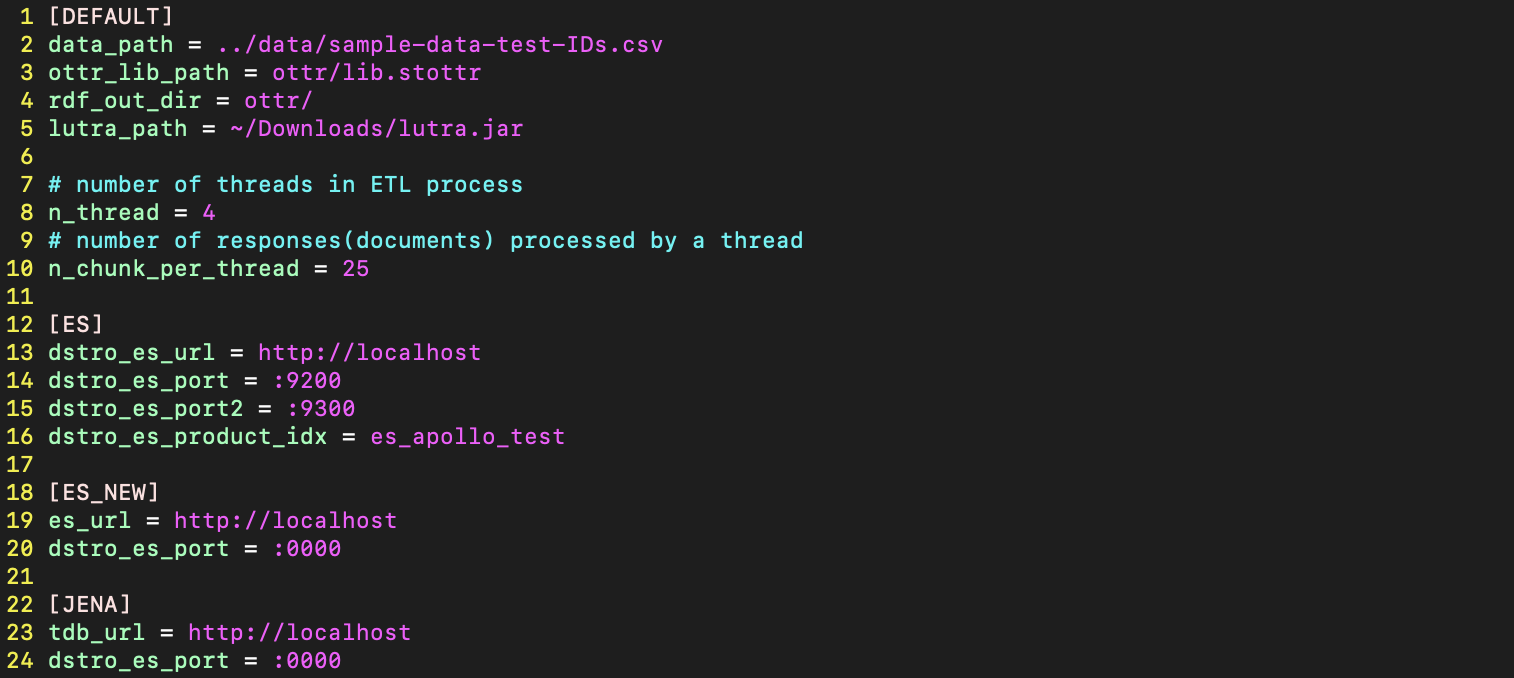
\includegraphics[width=0.75\textwidth]{../../resources/config_example.png}
	\caption{Configuration File example}
	\label{fig:config_example}
\end{figure}

The first four attributes can also be set with the help of environment variables. If neither 
environment variables are set nor configuration file misses some of the necessary attributes, 
program will halt with a self-descriptive error message.

\paragraph{Invalid Document Handling.}
As the extraction process of IDs have been implemented with 
\textit{regex}\footnote{Regular Expression} there are unittests to test edge cases. There are two 
cases: extracted ID is not a real ID or there is an ID which is not extracted. It is good to develop 
tests for each case.

\begin{table}[H]
	\centering
	\begin{tabular}{|p{0.45\textwidth}|p{0.45\textwidth}|}
		\hline
		\textbf{String} & \textbf{Is ID?} \\
		\hline
		10-23GGEZ-SHEESH & Yes \\
		\hline
		240V & Yes \\
		\hline
		10-23ggez-sheesh & No \\
		\hline
		800A & Yes \\
		\hline
		LCDAMOGUSRT34 & Yes \\
		\hline
	\end{tabular}
	\caption{Examples for ID verification}
	\label{tab:tests_id}
\end{table}

As shown in table \ref{tab:tests_id}, the first and the last strings are actual IDs whereas the third 
one is not. However, the second and the fourth strings are not real IDs either although our heuristic 
currently cannot classify such types correctly.

% \subsubsection{Performance}

% \begin{table}[H]
% 	\centering
% 	\begin{tabular}{|p{0.56\textwidth}|p{0.20\textwidth}|p{0.20\textwidth}|}
% 		\hline
% 		\textbf{Process} & \textbf{Run-time} & \textbf{Memory usage} \\
% 		\hline
% 		ESQuery (ETL-1 Extractor) & ? & ? \\
% 		\hline
% 		ES2TDB (ETL-1 Transformer) & ? & ? \\
% 		\hline
% 		TerminalOps (ETL-1 Loader) & ? & ? \\
% 		\hline
% 		Total (ETL-1) & ? & ? \\
% 		\hline
% 		\hline
% 		SPARQLQuery (ETL-2 Extractor) & ? & ? \\
% 		\hline
% 		TDB2ES (ETL-2 Transformer) & ? & ? \\
% 		\hline
% 		FileOps (ETL-2 Loader) & ? & ? \\
% 		\hline
% 		Total (ETL-2) & ? & ? \\
% 		\hline
% 	\end{tabular}
% 	\caption{Benchmark results for 100 documents}
% 	\label{tab:benchmark}
% \end{table}

\section{Discussion}

We can see that the developed software may still contain some bugs and terminate unexpectedly. This 
is due to several factors such as lack of unittests and edge cases given to the existing tests, 
poorly designed production and consumption of OperationalData objects, and imperfect heuristic 
implementation. In fact, the library and the software need to be improved furthermore. Several 
factors can be improved as shown below:

\begin{itemize}
	\item Heurictics can be added or modified according to SMEs knowledge
	\item More test cases for individual ETL operations can be added or even tests can be automated
	\item Data production and consumption can be handled with encapsulated furthermore
	\item Configuration file template can be structured more clearly
	\item Benchmarks can be designed to test the performance of each operation as well as the whole 
		to choose the best between different processing architectures
	\item etc.
\end{itemize}

We hope that the current software architecture, some core ideas about the pipeline components and 
processing paradigms and algorithms for them are not very far away from multiple future versions 
of the library and the software. Several modifications have to be made only on the implementational 
level and not on the architectural level.


% \chapter{Conclusion}								% 3 pages
\newpage
\section*{Conclusion}
\addcontentsline{toc}{section}{Conclusion}
\label{chap:conclusions}

\begin{enumerate}[wide=0pt]
% \section{On the use of ontologies}

\item Ontologies are used in different applications with mainly the unified goal of having a shared vocabulary 
with agreed-upon semantics. Such applications have emerged from domains such as fraud detection, 
web mining, search engines, legacy system integration, e-learning, data-level data integration, semantic 
publishing, and so on \cite{cmariakeet,ontotext}. You can imagine how having a shared vocabulary could 
potentially help to create more easily integratable systems and therefore, an ecosystem. Ontologies are 
very useful for such purposes.

\item Although developing and using ontologies can be very helpful for many real-world applications, they can 
also be painful to deal with in other areas of interest. The first problem is that it is not probably 
practically possible to define everything very rigorously by using some subset of the first-order logic. 
For example, how could one try to solve an image classification problem with the help of an ontology, or 
play chess, or solve a maze? Such problems require different solutions than using pure ontologies.
The second issue with using ontologies is that they have their own limitations in terms of the 
expressivity. To make the inference process tractable and decidable, there are different types of 
\textit{profiles} that are suitable for different use cases. The trade-off is obvious - more expressivity, 
less tractablity. For example, if you worked with the RDF framework, it would be impossible for you to 
express ``a class being a subclass of some another class'' since there is no such object property 
defined, and to be able to do it, RDFS would be one of the options to choose. However, as mentioned 
earlier, every framework has the trade-off between expressivity and tractability.

% \section{On the use of OTTR}

\item The idealogy behind OTTR is simple and powerful - \textit{using templates to build knowledge bases with 
better readability, maintainability and usability}. What it gives to its users is a more efficient 
process 
of dealing with ontologies and knowledge bases. Templates used in OTTR language prevent many potential 
repetitions by making the whole process more modular. Such separation between the design and the content 
allows one to develop a template library once and use it as much as needed to add new instances to the 
knowledge base.

Serialization of OTTR templates into RDF/OWL format is another benefit of using them. Imagine you have 
built a template library that can be used to add instances to the KB and the library itself could be 
loaded to the same KB. You would not need to store the library file separately on your local machine or 
some separate database than the one which contains the instances. So, the library file can be fetched 
from the same database either to check the validity of the triples or add new instances more reliably and 
easily.

% \section{Experiences gained during the internship}

\item To be able to solve the knowledge acquisition task, we encountered many problems along the way. These 
problems included thinking individually and brainstorming as a team with my supervisor. Communication 
and shared vocabulary played an important role during such times since when having a discussion about 
ontologies, people can easily misunderstand each other due to ambiguously defined and/or used words. 
However, because of such situations the need for rigor became very obvious to me. I understood the 
non-triviality of building a good ontology, building trustfulness by centeralization\footnote{KG has 
been built to play the role of single unified information source.}, decreasing performance issues 
when scaling up the database size, etc. These real-world problems made me realize the importance of 
scientific methods, differences between theory(thinking without constraints) and practice(engineering 
- thinking with constraints), communication and organization.
\end{enumerate}

% \section{Side notes}
% 
% Artificial Intelligence


\chapter*{About LITIS Laboratory}					% for ASOUI
\addcontentsline{toc}{chapter}{About LITIS Laboratory}
LITIS is a laboratory of the University of Havre Normandy, INSA Rouen Normandy and University of Rouen 
Normandy. The laboratory is a member of ``Digital Normandy'' which is the Norman network and the 
doctoral school of MIIS. LITIS is also a partner of the Normastic CNRS Research Federation. 
There are several research fields in LITIS which are shown below:

\begin{itemize}
	\item Information access
	\item Ambient intelligence
	\item Biomedical information processing
\end{itemize}

Beside the above shown fields of research, there are also several applications that are being 
addressed to by the work of laboratory workers:

\begin{itemize}
	\item Automotive and smart territories
	\item Information acces in all sectors
	\item Health
\end{itemize}

There are several departments in the laboratory each of which has expertise and works on different 
fields and aims at professional quality results. These fields are as shown below:

\begin{itemize}
	\item \textbf{Machine Learning}\newline
		Different techniques and/or models such as Markovian models, graph-based classification, 
		kernel machines, etc. are used in ML applications. Understanding and being able to use relevant 
		strategies is not a trivial job and the laboratory has theoretical and algorithmic expertise 
		on these domains.
	\item \textbf{Intelligent vehicle}\newline
		Transportation can become even efficient with the help of intelligent vehicles and other tools 
		used in everyday transit. Big data management for such intelligent transportation systems 
		plays an important role for this field of research.
	\item \textbf{Multi-agent systems}\newline
		Use of AI and Semantic Web technologies in order to automate decision-making processes through 
		reasoning and explainability is the main goal. This research field also focuses on the 
		human-machine interfaces for the development of socio-technical systems.
	\item \textbf{Health and Information Technology}\newline
		Analyzing biologcial data to gather relevant information in the field of bioinformatics. 
		Therapeutic monitoring and prediction in the domain of medical imaging is also a part of this 
		research field.
	\item \textbf{Combinatorics and Algorithms}\newline
		Having many applications in information processing such as words, automatons, free monoids, 
		etc., the members of this field focus on the study of models of algebraic nature to analyze 
		combinatorial and algorithmic aspects of them.
\end{itemize}

Besides scientific aspects and achievements of the LITIS laboratory, there are safety guidelines 
for emergency and those guidelines are practiced by the workers from time to time. In LITIS, 
researchers are very welcoming and they usually try to help each other on local social media channels 
when there is some technical problems to be solved. In my opinion, such attitude is one of the biggest 
achievements of the laboratory or even any company.

% The laboratory keeps close relations with Malaysia, Argentina, Canada, Brazil, China, Spain, 
% South Korea, The United States, Romania, Morocco, Italy and so on.
% LITIS also collaborates with many leading international groups such as Orange Labs, Airbus Defense and 
% Space, ITESOFT, bioMérieux, Peugeot PSA, Siemens, Valeo as well as some other small companies.

% \section{Interview}

% This interview has been taken from ??? who is currently an engineer working on ??? in the LITIS laboratory.

% \begin{table}[ht]
% 	\centering
% 	\begin{tabular}{p{0.1\textwidth}p{0.9\textwidth}}
% 		\hline
% 		\textbf{Q:} & What is intelligence? (is it reproducable by computation?) \\
% 		\textbf{A:} & ? \\
% 		\hline
% 		\textbf{Q:} & What is consciousness? (is it reproducable by computation?) \\
% 		\textbf{A:} & ? \\
% 		\hline
% 		\textbf{Q:} & We usually talk about the need for black box models to be explainable and so forth. 
% 		Up until now, full functionality of our brains have not been discoevered completely and there 
% 		are many puzzles waiting to be solved in the future. How do you think we ara capable of explaining 
% 		things without even acknowledging what is going on underneath? If our explainations are completely 
% 		the by-product of our brain activities, do you think that explainability could potentially emerge 
% 		from black-box or non-explainable models at some point? \\
% 		\textbf{A:} & ? \\
% 		\hline
% 		\textbf{Q:} & The problem-solving methodologies are developed either to deal with continuous or 
% 		discrete spaces. For example, problems related to Integer Programming, Boolean Satisfiability, 
% 		Domain-specific Language Search are inherently discrete whereas problems related to Linear 
% 		Regression, Artificial Neural Networks, Kernel Machines are continious by nature. What do you 
% 		think of the dichotonomy between ``discrete'' and ``continuous''? \\
% 		\textbf{A:} & ? \\
% 		\hline
% 		\textbf{Q:} & How do you think more generalization power could be achieved by the AI models 
% 		and do you think of (lossless) compression as generalization?
% 		\textbf{A:} & ? \\
% 		\hline
% 		\textbf{Q:} & If you had to classify your thoughts/works in AI, what category would you choose - 
% 		evolutionist, emergentist/reductionist, symbolist, connectionist, Bayesianist?
% 		\textbf{A:} & ? \\
% 		\hline
% 		\textbf{Q:} & What pieces do connectionism (i.e., ML/DL) lack in order to fully satisfy our 
% 		needs or achieve better problem solving abilities? \\
% 		\textbf{A:} & ? \\
% 		\hline
% 		\textbf{Q:} & What pieces do symbolism (i.e., expert systems) lack in order to fully satisfy 
% 		our needs or achieve better problem solving abilities? \\
% 		\textbf{A:} & ? \\
% 		\hline
% 		\textbf{Q:} & What type of architectures do you think will be used the most in the future? \\
% 		\textbf{A:} & ? \\
% 		\hline
% 		\textbf{Q:} & What would be your advice to the people working on your field? \\
% 		\textbf{A:} & ? \\
% 		\hline
% 	\end{tabular}
% 	\caption{Interview Q\&A}
% 	\label{tab:interview}
% \end{table}


% \chapter{References}								% 2 pages
% \bibliographystyle{unsrt}
\printbibliography

% \appendix
\chapter*{Appendices}								% 10 pages
\addcontentsline{toc}{chapter}{Appendices}
\section{Appendix A}
Ya-ya-ya-ya-ya!

\section{Appendix B}
Example


\end{document}
